\chapter{PENGUJIAN}
\label{sec:chap4_pengujian}
\vspace{1ex}

Bab ini menjelaskan prosedur pengujian yang dilakukan, rancangan eksperimen variasi parameter, serta cara interpretasi hasil evaluasi. Pengujian dirancang untuk menjawab empat pertanyaan utama: (1) seberapa baik performa sistem re-identifikasi penyu laut yang dibangun ketika berjalan pada satu konfigurasi acuan yang ditetapkan dari konvensi literatur, (2) sejauh mana dan ke arah mana setiap parameter mempengaruhi performa tersebut ketika divariasikan secara terkendali, (3) seberapa baik model bergeneralisasi apabila diterapkan pada dataset yang berbeda, di mana kondisi pengambilan citranya berbeda, dan (4) seberapa baik model dalam mengolah data identitas baru yang tidak terdaftar sebelumnya.

\section{Lingkungan Pengujian}
\subsection{Perangkat Keras dan Perangkat Lunak}

Seluruh eksperimen dijalankan pada lingkungan dengan spesifikasi sebagai berikut:

\begin{table}[ht]
    \centering
    \caption{Spesifikasi lingkungan pengujian}
    \label{tab:env}
    \renewcommand{\arraystretch}{1.25}
    \begin{tabular}{ll}
        \hline
        \textbf{Komponen} & \textbf{Spesifikasi}             \\
        \hline
        GPU               & \textit{NVIDIA GeForce RTX 4090} \\
        CPU               & \textit{Intel Core i9-13900KF}   \\
        RAM               & \textit{64 GB}                   \\
        Sistem Operasi    & \textit{Windows 11 Enterprise}   \\
        Python            & \textit{Python 3.10.11}          \\
        PyTorch           & \textit{torch 2.11.0+cu126}      \\
        timm              & \textit{timm 1.0.25}             \\
        \hline
    \end{tabular}
\end{table}

Untuk menjamin reproduktibilitas, seluruh eksperimen menggunakan \textit{random seed} yang tetap ($\texttt{SEED} = 42$) pada semua pustaka yang relevan (\texttt{random}, \texttt{numpy}, dan \texttt{torch}).

\section{Rancangan Eksperimen}
\subsection{Konfigurasi Acuan}
Sebelum melakukan variasi parameter, ditetapkan satu konfigurasi acuan (\textit{default}) yang menjadi titik referensi seluruh eksperimen. Konfigurasi ini ditetapkan berdasarkan nilai-nilai yang lazim pada literatur re-identifikasi berbasis ViT dan \textit{metric learning}, lalu disesuaikan dengan skala dataset SeaTurtleIDHeads. Penetapan acuan yang bersifat konvensional dan independen terhadap hasil eksperimen diperlukan agar analisis \textit{one-factor-at-a-time} (OFAT) tidak bersifat sirkular. Kontribusi setiap parameter hanya dapat dinilai secara objektif apabila titik acuannya ditentukan tanpa memanfaatkan informasi dari hasil variasi yang justru hendak dievaluasi. Seluruh parameter pada Tabel~\ref{tab:default} merupakan nilai \textit{default} yang digunakan.

\begin{table}[ht]
    \centering
    \caption{Konfigurasi acuan}
    \label{tab:default}
    \renewcommand{\arraystretch}{1.25}
    \begin{tabular}{llll}
        \hline
        \textbf{Kategori} & \textbf{Parameter}         & \textbf{Notasi}      & \textbf{Nilai Acuan} \\
        \hline
        Dataset           & Ukuran citra               & $\mathit{img\_size}$ & 256                  \\
                          & Citra galeri per identitas & $N_G$                & 3                    \\
        \hline
        Arsitektur        & Backbone                   &                      & ViT-B/16 DINOv3      \\
                          & Dimensi embedding          & $d_e$                & 256                  \\
                          & Dropout                    & $p_{\text{drop}}$    & 0{.}1                \\
        \hline
        Loss              & Skala ArcFace              & $s_a$                & 32{.}0               \\
                          & Margin ArcFace             & $m_a$                & 0{.}5                \\
                          & Margin Triplet             & $m_t$                & 0{.}3                \\
                          & Bobot Triplet              & $\lambda_t$          & 0{.}5                \\
        \hline
        Pelatihan         & Identitas per batch        & $P$                  & 16                   \\
                          & Citra per identitas        & $K$                  & 4                    \\
                          & Jumlah epoch               & $E$                  & 50                   \\
                          & Warmup epoch               & $W$                  & 5                    \\
                          & Gradient clipping          & $G_{\max}$           & 1{.}0                \\
                          & Patience early stopping    & $P_{\text{stop}}$    & 10 interval          \\
        \hline
        Optimizer         & Weight decay               & $\lambda_w$          & $10^{-4}$            \\
                          & Base learning rate         & $\eta_{\text{base}}$ & $10^{-3}$            \\
                          & Backbone base LR           & $\eta_{\text{bb}}$   & $10^{-5}$            \\
                          & Faktor peluruhan LR        & $\gamma$             & 0{.}75               \\
        \hline
    \end{tabular}
\end{table}

Penjelasan fungsi dan justifikasi pemilihan setiap nilai acuan diuraikan sebagai berikut:

\textbf{Dataset.} \textit{Ukuran citra} ($\mathit{img\_size}$) adalah resolusi citra masukan setelah proses \textit{resize}, yang menentukan jumlah token \textit{patch} yang diproses ViT sebesar $(\mathit{img\_size}/16)^2$ untuk \textit{patch} $16\times16$. Nilai acuan 256 dipilih sebagai kompromi antara detail spasial dan biaya komputasi: pada resolusi ini dihasilkan $16\times16=256$ token \textit{patch}, cukup rapat untuk menangkap pola sisik dan kontur kepala penyu tanpa beban komputasi resolusi yang lebih tinggi. \textit{Jumlah citra galeri per identitas} ($N_G$) menentukan berapa banyak citra tiap identitas yang dijadikan galeri dan di-\textit{mean-pool} menjadi satu vektor prototipe, sementara sisa citranya menjadi \textit{query}. Nilai acuan $N_G=3$ dipilih agar prototipe galeri cukup stabil sekaligus menyisakan cukup citra \textit{query} per identitas; nilai yang terlalu kecil membuat prototipe rentan \textit{noise}, sedangkan yang terlalu besar mengurangi jumlah identitas yang memenuhi ambang minimum citra.

\textbf{Arsitektur.} \textit{Backbone} adalah jaringan ekstraktor fitur (ViT DINOv3) yang mengubah citra menjadi representasi vektor, dengan varian \textit{Small}, \textit{Base}, dan \textit{Large} berbeda pada kedalaman, lebar, dan jumlah parameter. Varian ViT-B/16 dipilih sebagai titik tengah kapasitas: varian \textit{Small} berisiko kurang ekspresif untuk tugas \textit{fine-grained}, sedangkan \textit{Large} menuntut memori dan waktu yang jauh lebih besar; fitur \textit{self-supervised} DINOv3 yang diketahui kuat untuk representasi bertekstur halus membuat varian \textit{Base} memberikan keseimbangan kapasitas dan biaya yang wajar. \textit{Dimensi embedding} ($d_e$) adalah panjang vektor \textit{embedding} akhir hasil proyeksi fitur \textit{backbone}, yang menjadi ruang tempat \textit{cosine similarity} antar-citra dihitung. Nilai acuan 256 umum pada sistem re-identifikasi: cukup ringkas untuk menekan risiko \textit{overfitting} pada dataset berskala terbatas, namun cukup ekspresif untuk memisahkan identitas. \textit{Dropout} ($p_{\text{drop}}$) adalah probabilitas penonaktifan neuron secara acak selama pelatihan yang berfungsi sebagai regularisasi; nilai acuan 0.1 dipilih sebagai regularisasi ringan standar.

\textbf{Loss.} \textit{Skala ArcFace} ($s_a$) adalah faktor pengali pada logit \textit{cosine} sebelum \textit{softmax} yang mengontrol ketajaman distribusi probabilitas antar-kelas pada \textit{hypersphere}. Nilai acuan 32.0 sengaja dipilih lebih rendah dari nilai 64 pada formulasi ArcFace asli, karena jumlah identitas pada dataset ini jauh lebih sedikit dibanding dataset wajah berskala besar tempat nilai 64 lazim digunakan; skala yang lebih moderat memberikan distribusi sudut antar-kelas yang lebih sesuai dengan jumlah kelas yang kecil. \textit{Margin ArcFace} ($m_a$) adalah margin sudut aditif pada sudut terhadap kelas target yang memaksa separasi antar-identitas lebih lebar; nilai acuan 0.5 mengikuti \textit{default} formulasi ArcFace asli. \textit{Margin Triplet} ($m_t$) adalah jarak minimum yang diinginkan antara pasangan positif dan pasangan negatif dalam \textit{triplet loss}, sedangkan \textit{bobot Triplet} ($\lambda_t$) mengatur besar kontribusi \textit{Triplet Loss} pada fungsi \textit{loss} gabungan $\mathcal{L} = \mathcal{L}_{\text{ArcFace}} + \lambda_t \cdot \mathcal{L}_{\text{Triplet}}$. Nilai acuan $m_t=0{.}3$ dan $\lambda_t=0{.}5$ merupakan nilai umum pada skema gabungan ArcFace+Triplet, dengan $\lambda_t=0{.}5$ memberi bobot seimbang antara kedua komponen \textit{loss}.

\textbf{Pelatihan.} \textit{Identitas per batch} ($P$) dan \textit{citra per identitas} ($K$) merupakan pasangan parameter \textit{PK-sampling}: $P$ menentukan jumlah identitas berbeda per \textit{batch} dan $K$ jumlah citra per identitas, sehingga ukuran \textit{batch} efektif adalah $P \times K$. Komposisi acuan $P=16$ dan $K=4$ (\textit{batch size} 64) lazim untuk penambangan \textit{triplet}: $K=4$ menjamin tersedianya pasangan positif yang cukup untuk tiap identitas, sementara $P=16$ menjaga keberagaman identitas per iterasi dengan \textit{batch size} yang masih nyaman bagi memori GPU. \textit{Jumlah epoch} ($E$) adalah banyaknya lintasan penuh atas data pelatihan; nilai acuan 50 merupakan anggaran yang wajar untuk \textit{fine-tuning} \textit{backbone} terlatih pada dataset berukuran terbatas. \textit{Warmup epoch} ($W$) adalah jumlah \textit{epoch} awal ketika laju belajar dinaikkan bertahap sebelum jadwal \textit{cosine decay} aktif; nilai acuan 5 setara 10\% dari total \textit{epoch}, praktik standar untuk kestabilan awal pelatihan \textit{transformer}. \textit{Gradient clipping} ($G_{\max}$) adalah batas atas norma gradien untuk mencegah lonjakan pembaruan bobot, dan \textit{patience early stopping} ($P_{\text{stop}}$) adalah jumlah interval evaluasi tanpa perbaikan yang ditoleransi sebelum pelatihan dihentikan dini; nilai acuan $G_{\max}=1{.}0$ dan $P_{\text{stop}}=10$ interval merupakan nilai standar untuk menjaga kestabilan gradien dan menghentikan pelatihan tanpa terlalu prematur.

\textbf{Optimizer.} \textit{Weight decay} ($\lambda_w$) adalah koefisien regularisasi yang memberi penalti pada besarnya bobot untuk menekan kompleksitas model; nilai acuan $10^{-4}$ merupakan nilai regularisasi standar. \textit{Base learning rate} ($\eta_{\text{base}}$) adalah laju belajar untuk \textit{head} klasifikasi/\textit{metric learning} yang diinisialisasi acak, sedangkan \textit{backbone base LR} ($\eta_{\text{bb}}$) adalah laju belajar terpisah untuk \textit{backbone} terlatih. Nilai acuan $\eta_{\text{base}}=10^{-3}$ ditetapkan lebih tinggi karena \textit{head} perlu belajar lebih cepat, sedangkan $\eta_{\text{bb}}=10^{-5}$ sengaja jauh lebih kecil mengikuti praktik \textit{fine-tuning} konservatif yang menjaga fitur DINOv3 terlatih agar tidak rusak. \textit{Faktor peluruhan LR per layer} ($\gamma$) menerapkan \textit{layer-wise learning rate decay}, di mana laju belajar tiap \textit{layer} diskalakan dengan $\gamma$ pangkat kedalaman relatifnya sehingga \textit{layer} yang lebih dangkal (fitur lebih umum) menerima laju belajar lebih kecil; nilai acuan 0.75 umum pada \textit{fine-tuning} ViT. Perlu dicatat bahwa pilihan konservatif pada $\eta_{\text{bb}}$ kemudian terbukti menjadi salah satu pembatas performa terbesar pada pengujian variasi (Tabel~\ref{tab:var_bblr}). Temuan tersebut hanya dapat terungkap karena nilai acuannya ditetapkan berdasarkan konvensi, bukan berdasarkan hasil eksperimen.

\subsection{Protokol Evaluasi}
\label{subsec:protokol_evaluasi}

Setiap konfigurasi dievaluasi secara konsisten menggunakan protokol berikut:

\begin{enumerate}
    \item Model dilatih menggunakan data pelatihan SeaTurtleIDHeads. \textit{Checkpoint} terbaik dipilih berdasarkan nilai \textit{Rank-1} tertinggi pada data validasi. Apabila nilai \textit{Rank-1} sama, maka ditetapkan berdasarkan nilai \textit{Rank-5} tertinggi.
    \item Model terbaik dievaluasi menggunakan dataset SeaTurtleIDHeads dengan cakupan 10\% identitas terakhir yang tidak pernah dilihat model selama pelatihan.
    \item Performa dihitung dengan metrik \textit{Rank-1}, \textit{Rank-5}, \textit{Rank-10}, dan mAP menggunakan dua metode: \textit{cosine similarity} murni dan \textit{k-reciprocal re-ranking} ($k_1=20$, $k_2=6$, $\lambda_{\text{rr}}=0{.}3$).
    \item Ekstraksi \textit{embedding} dilakukan dengan satu kali lintasan maju (\textit{single-view}) atas citra yang telah di-\textit{resize}, tanpa \textit{test-time augmentation}. Vektor keluaran di-L2-\textit{normalize} sebelum perhitungan kemiripan.
\end{enumerate}

Istilah \textit{in-distribution} pada bab ini merujuk pada kesamaan domain pengambilan citra, yaitu dataset SeaTurtleIDHeads, dan bukan pada kesamaan identitas. Identitas pada data pengujian tetap terpisah sepenuhnya dari identitas pada data pelatihan, sehingga seluruh evaluasi bersifat \textit{open-set} pada level identitas.

\subsection{Variabel Parameter yang Diuji}

Penelitian ini menguji 19 parameter secara individual menggunakan pendekatan \textit{one-factor-at-a-time} (OFAT), yaitu satu parameter divariasikan sambil mempertahankan seluruh parameter lainnya pada nilai acuan. Pendekatan ini memungkinkan analisis kontribusi bersih dari setiap parameter terhadap performa sistem.

\begin{table}[H]
    \centering
    \caption{Variabel parameter yang diuji}
    \label{tab:params}
    \renewcommand{\arraystretch}{1.3}
    \begin{tabular}{p{2.8cm} p{3.5cm} p{2cm} p{4.5cm}}
        \hline
        \textbf{Kategori} & \textbf{Parameter}                               & \textbf{Default}  & \textbf{Nilai yang Diuji}                \\
        \hline
        \multirow{2}{*}{Dataset}
                          & $\mathit{img\_size}$                             & 256               & \{224, 320\}                             \\
                          & $N_G$ (\textit{n\_gallery})                      & 3                 & \{1, 5\}                                 \\
        \hline
        \multirow{3}{*}{Arsitektur}
                          & \textit{backbone}                                & ViT-B{/}16 DINOv3 & \{ViT-S{/}16 DINOv3, ViT-L{/}16 DINOv3\} \\
                          & $d_e$ (\textit{embed\_dim})                      & 256               & \{128, 512\}                             \\
                          & $p_{\text{drop}}$                                & 0{.}1             & \{0{.}0, 0{.}3\}                         \\
        \hline
        \multirow{4}{*}{Loss}
                          & $s_a$ (\textit{arcface\_scale})                  & 32{.}0            & \{16{.}0, 64{.}0\}                       \\
                          & $m_a$ (\textit{arcface\_margin})                 & 0{.}5             & \{0{.}3, \textbf{0{.}5}, 1{.}0, 2{.}0\}  \\
                          & $m_t$ (\textit{triplet\_margin})                 & 0{.}3             & \{0{.}1, \textbf{0{.}3}, 0{.}5\}         \\
                          & $\lambda_t$ (\textit{triplet\_weight})           & 0{.}5             & \{0{.}0, 0{.}2, \textbf{0{.}5}, 0{.}8\}  \\
        \hline
        \multirow{6}{*}{Pelatihan}
                          & $P$ (\textit{p\_identities})                     & 16                & \{8, 32\}                                \\
                          & $K$ (\textit{k\_images})                         & 4                 & \{2, 8\}                                 \\
                          & $E$ (\textit{num\_epoch})                        & 50                & \{30, 100\}                              \\
                          & $W$ (\textit{warmup\_epoch})                     & 5                 & \{3, 10\}                                \\
                          & $G_{\max}$ (\textit{grad\_clip})                 & 1{.}0             & \{0{.}5, 5{.}0\}                         \\
                          & $P_{\text{stop}}$ (\textit{patience})            & 10                & \{5, 20, 40\}                            \\
        \hline
        \multirow{4}{*}{Optimizer}
                          & $\lambda_w$ (\textit{weight\_decay})             & $10^{-4}$         & \{$10^{-5}$, $10^{-3}$\}                 \\
                          & $\eta_{\text{base}}$ (\textit{base\_lr})         & $10^{-3}$         & \{$10^{-4}$, $10^{-2}$\}                 \\
                          & $\eta_{\text{bb}}$ (\textit{backbone\_base\_lr}) & $10^{-5}$         & \{$10^{-6}$, $10^{-4}$\}                 \\
                          & $\gamma$ (\textit{lr\_decay})                    & 0{.}75            & \{0{.}65, 0{.}85\}                       \\
        \hline
    \end{tabular}
\end{table}

%% ============================================================
\section{Hasil Pengujian Acuan}
%% ============================================================

\subsection{Kurva Pelatihan}

Gambar~\ref{fig:training_curves} menampilkan kurva \textit{total loss} pelatihan dan metrik validasi (\textit{Rank-1} dan mAP) terhadap \textit{epoch}. Kurva tersebut diamati untuk memverifikasi tiga hal, yaitu (i) \textit{loss} menurun secara monoton tanpa lonjakan besar sebagai penanda pelatihan yang stabil, (ii) metrik validasi meningkat secara konsisten selama fase \textit{warmup} hingga \textit{cosine decay} aktif, dan (iii) tidak terdapat \textit{overfitting} yang signifikan, yaitu \textit{loss} validasi tidak meningkat drastis sementara \textit{loss} pelatihan terus menurun.

\begin{figure}[H]
    \centering
    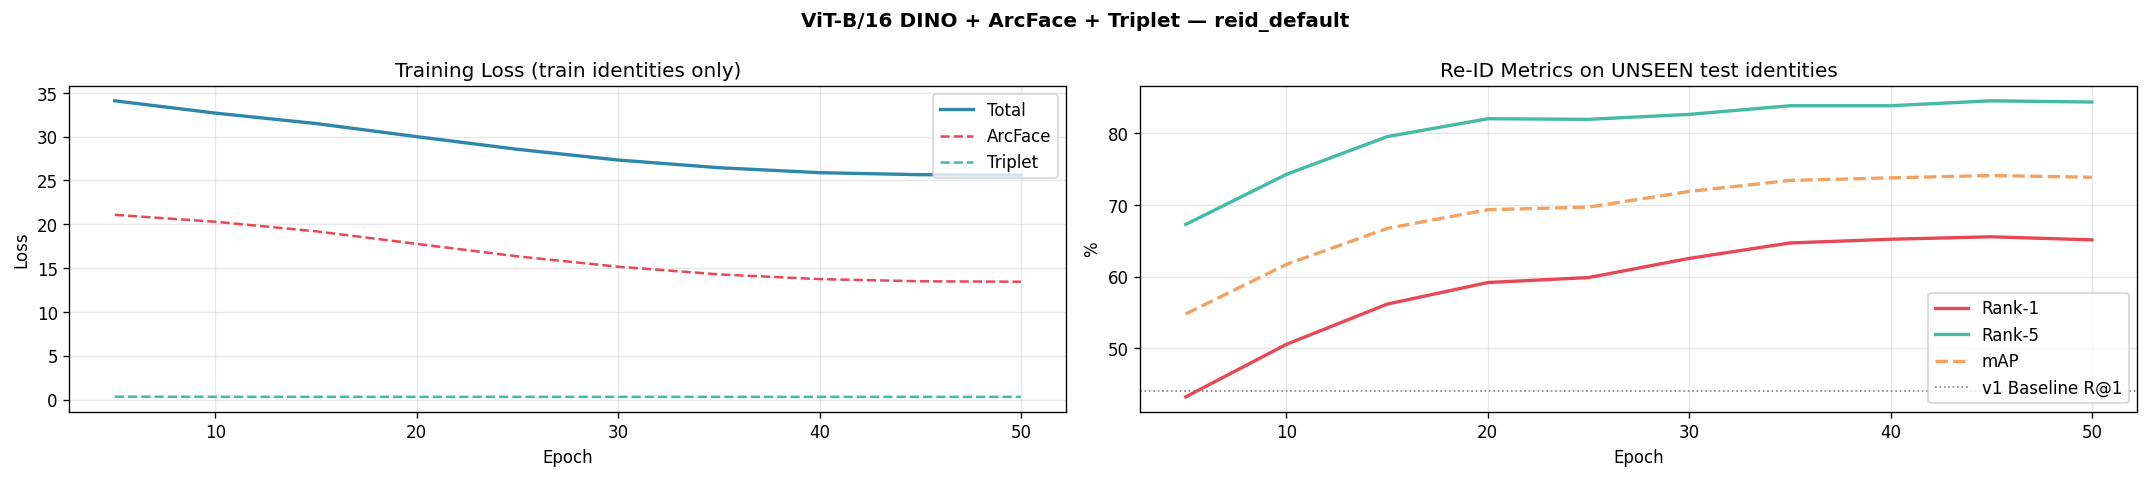
\includegraphics[width=\textwidth]{bab3/reid_default/training_curves.png}
    \caption{Kurva pelatihan konfigurasi acuan: (kiri) \textit{total loss} per \textit{epoch}; (kanan) \textit{Rank-1} dan mAP pada data validasi setiap 5 \textit{epoch}.}
    \label{fig:training_curves}
\end{figure}

% VERIFIKASI: cocokkan paragraf berikut dengan kurva aktual.
Ketiga kriteria tersebut terpenuhi pada konfigurasi acuan. \textit{Total loss} menurun secara monoton sepanjang 50 \textit{epoch} tanpa lonjakan, sehingga dapat disimpulkan bahwa kombinasi \textit{warmup} 5 \textit{epoch} dan \textit{gradient clipping} pada $G_{\max}=1{.}0$ memadai untuk menjaga kestabilan pelatihan. Metrik validasi meningkat tajam pada fase \textit{warmup}, kemudian melandai seiring aktifnya \textit{cosine decay} tanpa memperlihatkan penurunan pada \textit{epoch} akhir. Ketiadaan indikasi \textit{overfitting} pada anggaran $E=50$ ini konsisten dengan dua temuan yang diperoleh pada pengujian variasi, yaitu bahwa perpanjangan pelatihan hingga $E=100$ masih meningkatkan performa (Tabel~\ref{tab:var_epoch}) dan bahwa penambahan regularisasi justru menurunkan performa (Tabel~\ref{tab:var_dropout}). Dengan demikian dapat disimpulkan bahwa pada konfigurasi acuan model belum mencapai batas kapasitasnya, dan faktor pembatas utamanya adalah anggaran \textit{epoch}, bukan kekurangan regularisasi.

\subsection{Hasil Evaluasi Acuan}

Tabel~\ref{tab:baseline_results} menyajikan hasil evaluasi konfigurasi acuan pada dataset pengujian SeaTurtleIDHeads. Setiap metrik dilaporkan dua kali, yaitu menggunakan \textit{cosine similarity} murni (\textit{Cosine}) dan setelah \textit{k-reciprocal re-ranking} (\textit{+Re-rank}).

\begin{table}[H]
    \centering
    \caption{Hasil evaluasi konfigurasi acuan pada dataset pengujian SeaTurtleIDHeads}
    \label{tab:baseline_results}
    \renewcommand{\arraystretch}{1.35}
    \begin{tabular}{ l  c  c  c }
        \hline
        \textbf{Metrik} & \textbf{Cosine} & \textbf{+Re-rank} & \textbf{$\Delta$ (poin persentase)}                                                   \\
        \hline
        Rank-1  (\%)    & 77.4\%          & 78.3\%            & $+0{.}9$                                                                              \\
        Rank-5  (\%)    & 91.5\%          & 92.3\%            & $+0{.}8$                                                                              \\
        Rank-10 (\%)    & 95.9\%          & 95.1\%            & $-0{.}8$                                                                              \\
        mAP     (\%)    & 83.6\%          & 84.9\%            & $+1{.}3$                                                                              \\
        \hline
        \multicolumn{4}{l}{\footnotesize \textit{+Re-rank} = setelah k-reciprocal re-ranking ($k_1{=}20$, $k_2{=}6$, $\lambda_{\text{rr}}{=}0{.}3$).} \\
    \end{tabular}
\end{table}

\subsection{Analisis Hasil Acuan}

Berdasarkan hasil pada Tabel~\ref{tab:baseline_results}, beberapa observasi dapat dikemukakan.

\textbf{Pola antar-rank.} Akurasi meningkat seiring bertambahnya kedalaman peringkat yang ditoleransi, dengan pola perolehan yang menurun. Perpindahan dari \textit{Rank-1} ke \textit{Rank-5} memberikan peningkatan terbesar, yaitu dari 78.3\% menjadi 92.3\% atau sebesar 14.0 poin persentase, sedangkan perpindahan dari \textit{Rank-5} ke \textit{Rank-10} menghasilkan peningkatan yang jauh lebih kecil, yaitu dari 92.3\% menjadi 95.1\% atau sebesar 2.8 poin persentase. Pola tersebut memiliki implikasi praktis. Pada sekitar 14\% \textit{query}, identitas yang benar sesungguhnya telah berada di dalam lima kandidat teratas namun kalah tipis pada peringkat pertama, sehingga kegagalan model umumnya berupa kesalahan pengurutan pada peringkat teratas dan bukan kegagalan menemukan identitas yang benar. Sisa 4.9\% \textit{query} yang tetap gagal hingga \textit{Rank-10} merupakan kasus yang identitas benarnya memang tidak terjangkau, dan analisis kualitatif pada Subbab~\ref{subsec:kualitatif_id} menunjukkan bahwa kasus tersebut terkonsentrasi pada citra berkualitas rendah.

\textbf{Kontribusi re-ranking.} Efek \textit{k-reciprocal re-ranking} terhadap konfigurasi acuan bersifat positif namun tidak seragam. Pada \textit{Rank-1}, \textit{Rank-5}, dan mAP, re-ranking memberikan peningkatan masing-masing sebesar 0.9, 0.8, dan 1.3 poin persentase, yang menandakan bahwa struktur hubungan timbal balik antar tetangga dalam ruang \textit{embedding} berhasil dieksploitasi sebagai tahap pasca-proses tanpa biaya pelatihan tambahan. Sebaliknya, pada \textit{Rank-10} re-ranking sedikit menurunkan performa, yaitu dari 95.9\% menjadi 95.1\%. Pola tersebut wajar terjadi karena re-ranking mengoptimalkan konsistensi tetangga terdekat, sehingga paling menguntungkan pada peringkat teratas dan pada metrik agregat seperti mAP, sembari sesekali menggeser kandidat benar keluar dari rentang \textit{Rank-10} pada sebagian kecil \textit{query}. Perolehan bersihnya tetap positif, terutama pada mAP yang merupakan metrik paling representatif terhadap kualitas \textit{ranking} secara keseluruhan.

\subsection{Visualisasi t-SNE}

Gambar~\ref{fig:tsne} menampilkan visualisasi t-SNE dari vektor \textit{embedding} 20 identitas teratas pada data pengujian \textit{in-distribution}. Pengelompokan (\textit{clustering}) yang baik di ruang t-SNE, yaitu titik-titik dari identitas yang sama berdekatan dan terpisah dari identitas lain, mengkonfirmasi bahwa model berhasil membangun ruang \textit{embedding} yang diskriminatif.

\begin{figure}[H]
    \centering
    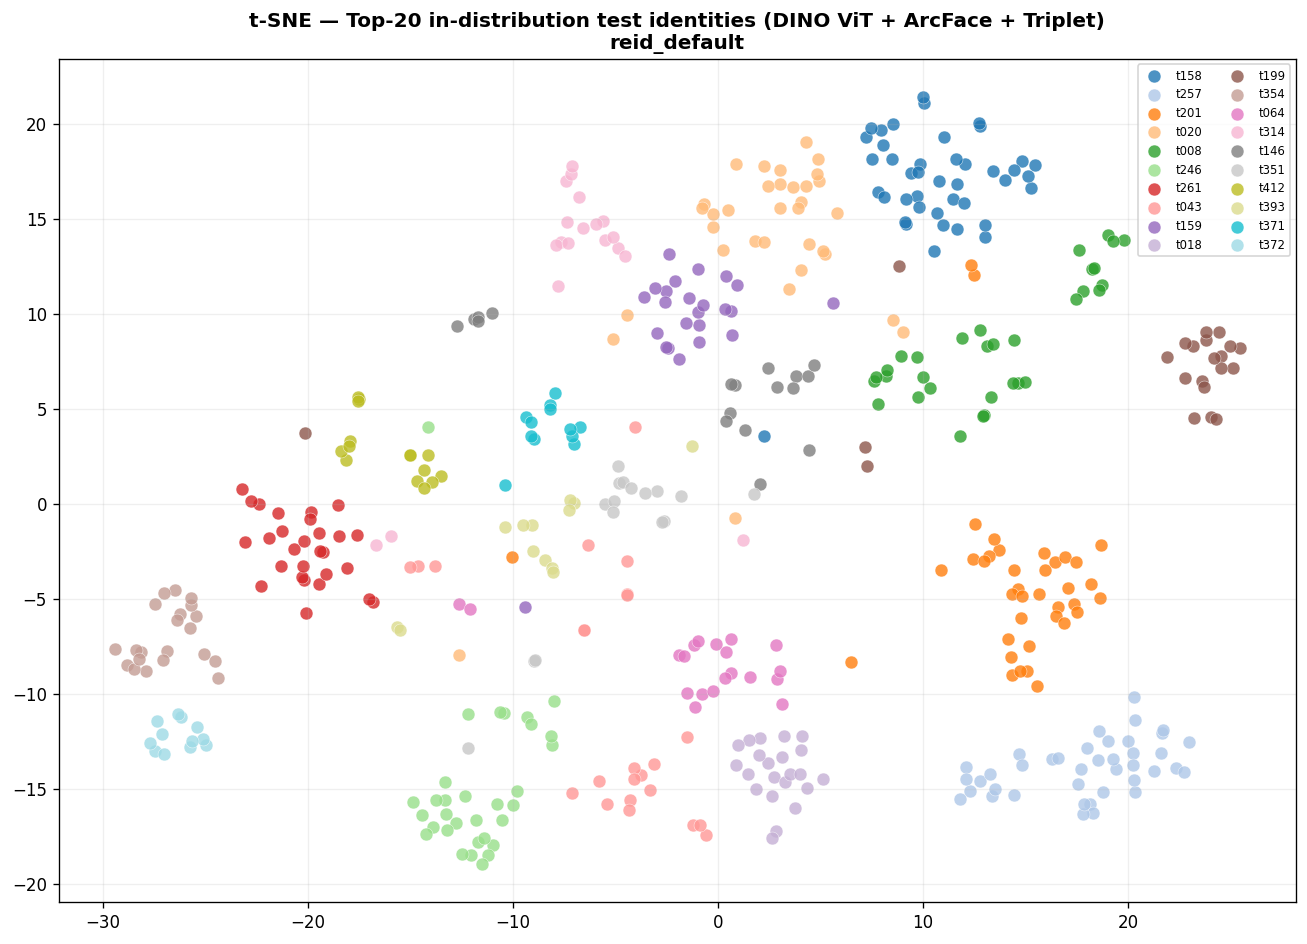
\includegraphics[width=0.85\textwidth]{bab4/tsne.png}
    \caption{Visualisasi t-SNE untuk 20 identitas penyu teratas pada data pengujian \textit{in-distribution}. Setiap warna mewakili satu identitas.}
    \label{fig:tsne}
\end{figure}

\subsection{Analisis Kualitatif Hasil Retrieval}
\label{subsec:kualitatif_id}

Gambar~\ref{fig:query_retrieval} menampilkan hasil \textit{retrieval} lima peringkat teratas untuk beberapa \textit{query} pada data pengujian \textit{in-distribution}, lengkap dengan skor \textit{cosine similarity} masing-masing kandidat.

\begin{figure}[H]
    \centering
    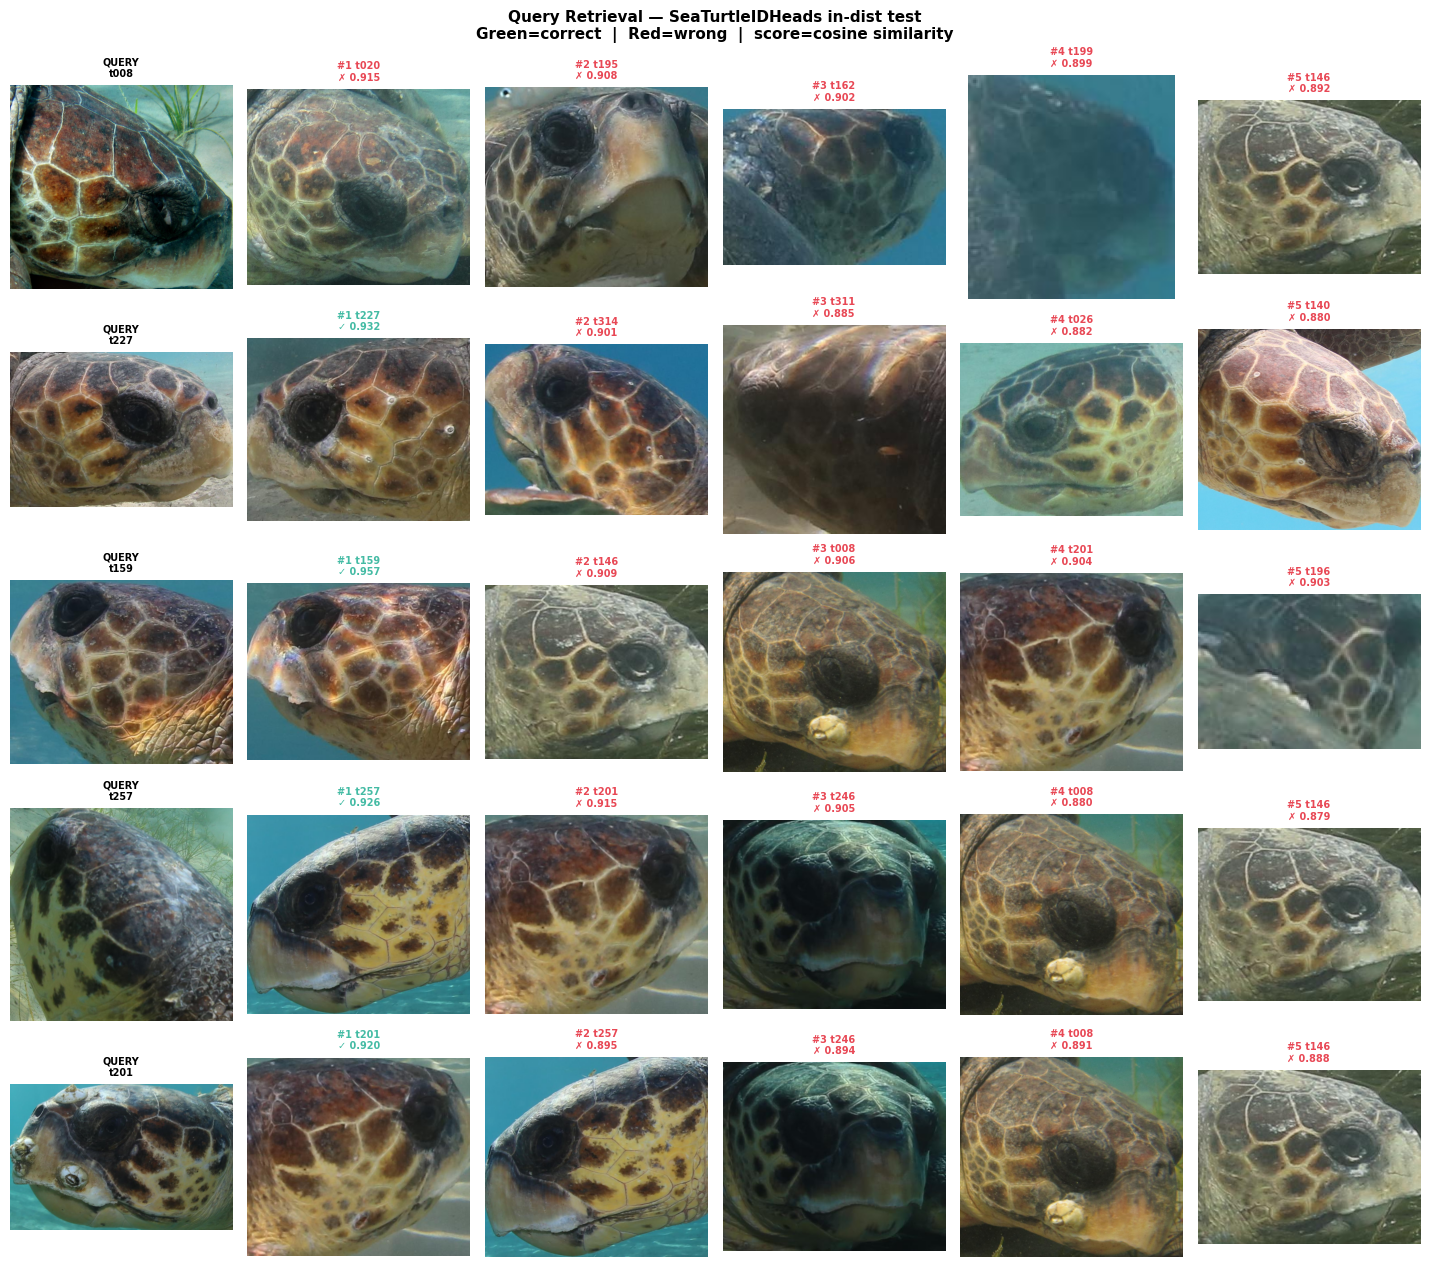
\includegraphics[width=\textwidth]{bab4/query_retrieval.png}
    \caption{Hasil \textit{retrieval} lima peringkat teratas pada data pengujian \textit{in-distribution} SeaTurtleIDHeads. Kolom pertama adalah citra \textit{query}, kolom berikutnya adalah kandidat galeri terurut menurun berdasarkan \textit{cosine similarity}. Hijau menandai identitas yang benar, merah menandai identitas yang salah.}
    \label{fig:query_retrieval}
\end{figure}

Dari Gambar~\ref{fig:query_retrieval} dapat dilihat bahwa pada \textit{query} yang berhasil (t227, t159, dan t257), kandidat peringkat-1 memperoleh skor yang jelas lebih tinggi daripada kandidat berikutnya, yaitu 0.932, 0.957, dan 0.926 terhadap kandidat kedua yang berada di sekitar 0.90. Hal ini menandakan bahwa model menemukan identitas yang benar dengan tingkat keyakinan yang terpisah dari kandidat pesaingnya.

Pengamatan pada kasus kegagalan menunjukkan bahwa kandidat yang keliru umumnya merupakan citra dengan pose kepala dan pencahayaan yang serupa dengan \textit{query}, atau citra yang buram dan berkontras rendah, misalnya kandidat \#3 dan \#4 pada baris t008. Hal ini mengindikasikan bahwa sisa kegagalan model terkonsentrasi pada citra berkualitas rendah, yaitu ketika pola sisik sebagai penanda identitas tidak lagi terbaca dengan jelas.

%% ============================================================
\section{Hasil Pengujian Variasi Parameter}
%% ============================================================

Bagian ini menyajikan hasil eksperimen variasi setiap parameter secara individual untuk menganalisis arah dan besar dampaknya terhadap performa. Metrik utama yang digunakan untuk perbandingan adalah \textit{Rank-1} dan mAP pada dataset pengujian SeaTurtleIDHeads dengan \textit{k-reciprocal re-ranking}. Untuk setiap parameter, fokus analisis diarahkan pada arah perubahan performa relatif terhadap acuan dan pada sensitivitas sistem terhadap parameter tersebut.

\subsection{Variasi Parameter Dataset}

\subsubsection{Ukuran Citra (\textit{img\_size})}

\begin{table}[H]
    \centering
    \caption{Pengaruh ukuran citra terhadap performa (+Re-rank)}
    \label{tab:var_imgsize}
    \renewcommand{\arraystretch}{1.25}
    \begin{tabular}{ccccc}
        \hline
        $\mathit{img\_size}$ & \textbf{Rank-1 (\%)} & \textbf{Rank-5 (\%)} & \textbf{Rank-10 (\%)} & \textbf{mAP (\%)} \\
        \hline
        224                  & 73.3\%               & 91.5\%               & 94.9\%                & 81.9\%            \\
        \textbf{256}         & 78.3\%               & 92.3\%               & 95.1\%                & 84.9\%            \\
        320                  & 76.1\%               & 92.5\%               & 96.0\%                & 84.9\%            \\
        \hline
    \end{tabular}
\end{table}

Berdasarkan hasil pengujian tersebut, pengaruh resolusi citra terhadap performa tidak bersifat monoton. Peningkatan resolusi dari 224 ke 256 (acuan) meningkatkan seluruh metrik secara jelas, dengan Rank-1 naik sebesar 5.0 poin persentase. Namun peningkatan lebih lanjut ke 320 tidak lagi memberikan perbaikan yang konsisten, yaitu Rank-1 justru menurun menjadi 76.1\% atau di bawah acuan 78.3\%, meskipun Rank-5, Rank-10, dan mAP sedikit lebih tinggi atau setara. Dengan mempertimbangkan bahwa resolusi yang lebih tinggi menuntut kebutuhan komputasi yang lebih besar tanpa keunggulan yang meyakinkan pada Rank-1, resolusi 256 dipertahankan sebagai nilai acuan yang memberikan keseimbangan terbaik antara performa dan biaya komputasi.

\subsubsection{Jumlah Citra Galeri per Identitas (\textit{n\_gallery})}

\begin{table}[H]
    \centering
    \caption{Pengaruh jumlah citra galeri per identitas terhadap performa (+Re-rank)}
    \label{tab:var_ngallery}
    \renewcommand{\arraystretch}{1.25}
    \begin{tabular}{ccccc}
        \hline
        $N_G$      & \textbf{Rank-1 (\%)} & \textbf{Rank-5 (\%)} & \textbf{Rank-10 (\%)} & \textbf{mAP (\%)} \\
        \hline
        1          & 58.2\%               & 83.9\%               & 92.8\%                & 69.3\%            \\
        \textbf{3} & 78.3\%               & 92.3\%               & 95.1\%                & 84.9\%            \\
        5          & 69.5\%               & 90.4\%               & 93.6\%                & 78.3\%            \\
        \hline
    \end{tabular}
\end{table}

Berdasarkan data tersebut, $N_G=3$ menghasilkan performa tertinggi, diikuti oleh $N_G=5$ dan $N_G=1$. Secara teoretis, $N_G=5$ diharapkan menghasilkan prototipe yang paling stabil dan karenanya performa tertinggi. Penurunan yang teramati berasal dari efek samping konstruksi \textit{split}, yaitu bertambahnya $N_G$ menaikkan ambang minimum citra per identitas sehingga jumlah identitas yang memenuhi syarat berkurang, sekaligus mengurangi jumlah citra \textit{query} yang tersisa. Perlu ditegaskan bahwa karena komposisi \textit{query} dan galeri berubah antar-nilai $N_G$, ketiga baris pada tabel tersebut tidak dievaluasi pada himpunan \textit{query} yang identik. Perbandingan antar-baris karenanya bersifat indikatif terhadap konfigurasi sistem secara keseluruhan, dan bukan merupakan perbandingan performa model murni pada tugas yang sama.

\subsection{Variasi Parameter Arsitektur}

\subsubsection{Backbone}

\begin{table}[H]
    \centering
    \caption{Pengaruh pemilihan backbone terhadap performa (+Re-rank)}
    \label{tab:var_backbone}
    \renewcommand{\arraystretch}{1.25}
    \begin{tabular}{lcccc}
        \hline
        \textbf{Backbone} & \textbf{Rank-1 (\%)} & \textbf{Rank-5 (\%)} & \textbf{Rank-10 (\%)} & \textbf{mAP (\%)} \\
        \hline
        ViT-S/16          & 61.4\%               & 82.1\%               & 91.0\%                & 70.3\%            \\
        \textbf{ViT-B/16} & 78.3\%               & 92.3\%               & 95.1\%                & 84.9\%            \\
        ViT-L/16          & 80.4\%               & 94.4\%               & 96.2\%                & 86.6\%            \\
        \hline
    \end{tabular}
\end{table}

Performa meningkat secara konsisten seiring bertambahnya ukuran \textit{backbone}, dari ViT-S/16 hingga ViT-L/16, pada seluruh metrik yang diukur. Peningkatan dari ViT-S/16 ke ViT-B/16 tergolong besar, yaitu Rank-1 naik sebesar 16.9 poin persentase, sedangkan peningkatan dari ViT-B/16 ke ViT-L/16 jauh lebih moderat, yaitu Rank-1 naik sebesar 2.1 poin persentase. Hal ini menunjukkan bahwa kapasitas representasi \textit{backbone} yang lebih besar membantu membedakan identitas penyu secara lebih baik, meskipun disertai \textit{diminishing return} yang tajam serta konsekuensi kebutuhan komputasi dan memori yang jauh lebih besar pada ViT-L/16.

\subsubsection{Dimensi Embedding (\textit{embed\_dim})}

\begin{table}[H]
    \centering
    \caption{Pengaruh dimensi embedding terhadap performa (+Re-rank)}
    \label{tab:var_embeddim}
    \renewcommand{\arraystretch}{1.25}
    \begin{tabular}{ccccc}
        \hline
        $d_e$        & \textbf{Rank-1 (\%)} & \textbf{Rank-5 (\%)} & \textbf{Rank-10 (\%)} & \textbf{mAP (\%)} \\
        \hline
        128          & 76.5\%               & 92.1\%               & 95.3\%                & 84.0\%            \\
        \textbf{256} & 78.3\%               & 92.3\%               & 95.1\%                & 84.9\%            \\
        512          & 76.6\%               & 92.1\%               & 94.7\%                & 83.9\%            \\
        \hline
    \end{tabular}
\end{table}

Ketiga nilai dimensi \textit{embedding} yang diuji menghasilkan performa yang berdekatan, dengan selisih Rank-1 tidak lebih dari 1.8 poin persentase dan selisih mAP tidak lebih dari 1.0 poin persentase. Hal ini menandakan bahwa sistem relatif robust terhadap parameter tersebut. Meski demikian, terdapat pola \textit{inverted-U}, yaitu $d_e=256$ memberikan performa terbaik pada Rank-1 (78.3\%) dan mAP (84.9\%), sementara dimensi yang lebih kecil ($d_e=128$) maupun yang lebih besar ($d_e=512$) sama-sama menurunkan performa hingga ke tingkat yang nyaris identik (Rank-1 76.5\% berbanding 76.6\%). Secara teoretis kedua penurunan tersebut berasal dari mekanisme yang berlawanan. Dimensi 128 terlalu ringkas untuk memisahkan identitas penyu yang bersifat \textit{fine-grained} sehingga kehilangan daya ekspresif, sedangkan dimensi 512 menambah kapasitas berlebih yang rentan \textit{overfitting} pada dataset berskala terbatas tanpa memberikan informasi diskriminatif tambahan. Perlu dicatat bahwa selisih sebesar itu berada pada orde beberapa \textit{query} saja, sehingga pola \textit{inverted-U} tersebut sebaiknya dibaca sebagai indikasi ketidakpekaan sistem terhadap $d_e$ dan bukan sebagai bukti kuat adanya titik optimum. Efeknya pun terkonsentrasi pada Rank-1 dan mAP, sedangkan Rank-5 dan Rank-10 hampir tidak berubah antar-nilai, dengan Rank-5 berada pada rentang 92.1\% hingga 92.3\%. Dengan demikian $d_e=256$ dipertahankan sebagai acuan.

\subsubsection{Dropout}

\begin{table}[H]
    \centering
    \caption{Pengaruh dropout terhadap performa (+Re-rank)}
    \label{tab:var_dropout}
    \renewcommand{\arraystretch}{1.25}
    \begin{tabular}{ccccc}
        \hline
        $p_{\text{drop}}$ & \textbf{Rank-1 (\%)} & \textbf{Rank-5 (\%)} & \textbf{Rank-10 (\%)} & \textbf{mAP (\%)} \\
        \hline
        0{.}0            & 81.0\%               & 91.7\%               & 94.9\%                & 86.0\%             \\
        \textbf{0{.}1}    & 78.3\%               & 92.3\%               & 95.1\%                & 84.9\%            \\
        0{.}3             & 73.1\%               & 90.8\%               & 95.1\%                & 81.2\%            \\
        \hline
    \end{tabular}
\end{table}

Berbeda dengan ekspektasi umum bahwa \textit{dropout} membantu regularisasi, performa pada pengujian ini justru menurun secara monoton seiring bertambahnya $p_{\text{drop}}$. Nilai $p_{\text{drop}}=0{.}0$ memberikan performa terbaik pada Rank-1 (81.0\%) dan mAP (86.0\%), keduanya lebih tinggi daripada acuan $p_{\text{drop}}=0{.}1$, sedangkan $p_{\text{drop}}=0{.}3$ menurunkan Rank-1 secara tajam hingga 73.1\%. Pola tersebut mengindikasikan bahwa model tidak berada pada rezim \textit{overfitting} yang membutuhkan regularisasi \textit{dropout}; sebaliknya, penonaktifan neuron secara acak justru membuang kapasitas representasi yang masih berguna. Temuan ini konsisten dengan hasil pada bobot Triplet Loss (Tabel~\ref{tab:var_tripletweight}) dan \textit{weight decay} (Tabel~\ref{tab:var_wd}), yang sama-sama menunjukkan bahwa regularisasi tambahan cenderung tidak menguntungkan pada konfigurasi ini, kemungkinan besar karena fitur \textit{self-supervised} DINOv3 yang telah terlatih sudah berperan sebagai regularisasi implisit yang kuat. Terdapat satu catatan penimbang, yaitu pada $p_{\text{drop}}=0{.}0$ nilai Rank-5 dan Rank-10 sedikit lebih rendah dibandingkan acuan, dengan Rank-5 sebesar 91.7\% berbanding 92.3\%, sehingga keunggulan penonaktifan \textit{dropout} paling terasa pada presisi teratas (Rank-1) dan pada metrik agregat (mAP). Meskipun data mendukung $p_{\text{drop}}=0{.}0$, penonaktifan \textit{dropout} sepenuhnya berpotensi meningkatkan risiko \textit{overfitting} pada skenario data yang lebih sempit, sehingga nilai tersebut menjadi kandidat kuat namun tetap perlu diverifikasi bersama parameter lain.

\subsection{Variasi Parameter Loss}

\subsubsection{Skala ArcFace (\textit{arcface\_scale})}

\begin{table}[H]
    \centering
    \caption{Pengaruh skala ArcFace terhadap performa (+Re-rank)}
    \label{tab:var_arcscale}
    \renewcommand{\arraystretch}{1.25}
    \begin{tabular}{ccccc}
        \hline
        $s_a$           & \textbf{Rank-1 (\%)} & \textbf{Rank-5 (\%)} & \textbf{Rank-10 (\%)} & \textbf{mAP (\%)} \\
        \hline
        16{.}0          & 72.9\%               & 91.9\%               & 94.9\%                & 81.7\%            \\
        \textbf{32{.}0} & 78.3\%               & 92.3\%               & 95.1\%                & 84.9\%            \\
        64{.}0          & 76.6\%               & 91.1\%               & 94.7\%                & 83.3\%            \\
        \hline
    \end{tabular}
\end{table}

Pengaruh skala ArcFace terhadap performa membentuk pola \textit{inverted-U} dengan puncak pada nilai acuan $s_a=32{.}0$. Penurunan skala ke 16.0 menurunkan seluruh metrik, khususnya Rank-1 yang turun sebesar 5.4 poin persentase dan mAP sebesar 3.2 poin persentase. Skala yang terlalu kecil membuat distribusi \textit{softmax} atas logit sudut menjadi terlalu landai, sehingga separasi antar-kelas melemah dan gradien tidak cukup menekan pemisahan identitas yang mirip. Sebaliknya, peningkatan skala ke 64.0 juga menurunkan performa dibandingkan acuan, yaitu Rank-1 sebesar 76.6\% dan mAP sebesar 83.3\%, meskipun tetap lebih baik daripada skala 16.0. Skala yang terlalu besar membuat logit menjadi terlalu tajam dan mudah jenuh sehingga gradien menjadi runcing dan optimisasi kurang stabil, dan efek tersebut diperberat oleh jumlah kelas yang sedikit pada dataset ini. Hasil tersebut mengonfirmasi justifikasi pemilihan acuan, yaitu bahwa nilai 64 yang lazim pada dataset wajah berskala besar memang kurang sesuai untuk jumlah identitas yang jauh lebih kecil pada penelitian ini, dan skala moderat 32.0 memberikan ketajaman distribusi sudut yang paling seimbang.

\subsubsection{Margin ArcFace (\textit{arcface\_margin})}

\begin{table}[H]
    \centering
    \caption{Pengaruh margin ArcFace terhadap performa (+Re-rank)}
    \label{tab:var_arcmargin}
    \renewcommand{\arraystretch}{1.25}
    \begin{tabular}{ccccc}
        \hline
        $m_a$          & \textbf{Rank-1 (\%)} & \textbf{Rank-5 (\%)} & \textbf{Rank-10 (\%)} & \textbf{mAP (\%)} \\
        \hline
        0{.}3         & 77.2\%               & 91.7\%               & 94.7\%                & 84.1\%             \\
        \textbf{0{.}5} & 78.3\%               & 92.3\%               & 95.1\%                & 84.9\%            \\
        1{.}0          & 80.0\%               & 92.1\%               & 95.3\%                & 85.8\%            \\
        2{.}0          & 76.5\%               & 91.1\%               & 94.4\%                & 83.7\%            \\
        \hline
    \end{tabular}
\end{table}

Performa terbaik justru dicapai pada $m_a=1{.}0$, yaitu sedikit lebih tinggi dibandingkan nilai acuan $m_a=0{.}5$, dengan Rank-1 sebesar 80.0\% berbanding 78.3\% dan mAP sebesar 85.8\% berbanding 84.9\%. Namun ketika margin diperbesar lebih lanjut menjadi $m_a=2{.}0$, performa menurun hingga di bawah nilai acuan. Pola tersebut menunjukkan adanya titik optimal margin, yaitu margin yang cukup besar untuk memberikan separasi antar-kelas yang kuat namun tidak terlalu besar sehingga menyulitkan konvergensi optimisasi ArcFace.

\subsubsection{Margin Triplet (\textit{triplet\_margin})}

\begin{table}[H]
    \centering
    \caption{Pengaruh margin Triplet terhadap performa (+Re-rank)}
    \label{tab:var_tripletmargin}
    \renewcommand{\arraystretch}{1.25}
    \begin{tabular}{ccccc}
        \hline
        $m_t$          & \textbf{Rank-1 (\%)} & \textbf{Rank-5 (\%)} & \textbf{Rank-10 (\%)} & \textbf{mAP (\%)} \\
        \hline
        0{.}1         & 76.5\%               & 91.5\%               & 95.1\%                & 83.6\%             \\
        \textbf{0{.}3} & 78.3\%               & 92.3\%               & 95.1\%                & 84.9\%            \\
        0{.}5          & 78.0\%               & 92.3\%               & 95.5\%                & 84.6\%            \\
        \hline
    \end{tabular}
\end{table}

Perbedaan performa antar nilai margin Triplet relatif kecil dibandingkan parameter lain, yang mengindikasikan bahwa sistem tidak terlalu sensitif terhadap parameter tersebut. Margin yang lebih besar ($m_t=0{.}5$) memberikan Rank-10 yang sedikit lebih baik, sementara margin yang lebih kecil ($m_t=0{.}1$) sedikit menurunkan performa Rank-1 dan mAP, namun secara keseluruhan selisihnya tidak lebih dari 1.8 poin persentase pada setiap metrik. Ketidakpekaan tersebut konsisten dengan temuan pada bobot Triplet (Tabel~\ref{tab:var_tripletweight}), yaitu apabila kontribusi Triplet Loss terhadap performa memang kecil atau bahkan negatif, maka wajar apabila penyetelan marginnya juga berdampak minim.

\subsubsection{Bobot Triplet (\textit{triplet\_weight})}

\begin{table}[H]
    \centering
    \caption{Pengaruh bobot Triplet Loss terhadap performa (+Re-rank)}
    \label{tab:var_tripletweight}
    \renewcommand{\arraystretch}{1.25}
    \begin{tabular}{ccccc}
        \hline
        $\lambda_t$     & \textbf{Rank-1 (\%)} & \textbf{Rank-5 (\%)} & \textbf{Rank-10 (\%)} & \textbf{mAP (\%)} \\
        \hline
        0{.}00          & 83.4\%               & 94.5\%               & 97.6\%                & 88.4\%            \\
        0{.}20          & 80.6\%               & 92.1\%               & 96.0\%                & 86.6\%            \\
        \textbf{0{.}50} & 78.3\%               & 92.3\%               & 95.1\%                & 84.9\%            \\
        0{.}80          & 77.6\%               & 91.9\%               & 95.3\%                & 84.1\%            \\
        \hline
    \end{tabular}
\end{table}

Performa tertinggi justru dicapai ketika Triplet Loss tidak diikutsertakan sama sekali ($\lambda_t=0{.}0$), yaitu dengan Rank-1 sebesar 83.4\% dan mAP sebesar 88.4\%, keduanya lebih tinggi dibandingkan konfigurasi acuan. Performa menurun secara monoton pada seluruh metrik seiring bertambahnya bobot Triplet Loss. Hal ini mengindikasikan bahwa pada konfigurasi dan skala dataset ini, ArcFace Loss saja sudah cukup diskriminatif, sementara penambahan Triplet Loss justru mengganggu proses optimisasi. Temuan tersebut memiliki implikasi lanjutan, yaitu karena $\lambda_t=0{.}0$ menonaktifkan Triplet Loss sepenuhnya, komposisi \textit{PK-sampling} ($P$ dan $K$) kehilangan justifikasi utamanya sebagai penjamin ketersediaan pasangan positif untuk penambangan \textit{triplet}. Hal ini menjelaskan mengapa $K=2$ justru mengungguli $K=4$ pada Tabel~\ref{tab:var_batch}.

\subsection{Variasi Parameter Pelatihan}

\subsubsection{Komposisi Batch: Identitas per Batch ($P$) dan Citra per Identitas ($K$)}

\begin{table}[H]
    \centering
    \caption{Pengaruh komposisi batch terhadap performa (+Re-rank)}
    \label{tab:var_batch}
    \renewcommand{\arraystretch}{1.25}
    \begin{tabular}{cccccc}
        \hline
        $P$         & $K$        & \textbf{Batch Size} & \textbf{Rank-1 (\%)} & \textbf{Rank-5 (\%)} & \textbf{mAP (\%)} \\
        \hline
        8           & \textbf{4} & 32                  & 79.1\%               & 92.1\%               & 85.5\%            \\
        \textbf{16} & \textbf{4} & \textbf{64}         & 78.3\%               & 92.3\%               & 84.9\%            \\
        32          & \textbf{4} & 128                 & 68.5\%               & 88.7\%               & 78.2\%            \\
        \textbf{16} & 2          & 32                  & 79.1\%               & 95.3\%               & 86.3\%            \\
        \textbf{16} & 8          & 128                 & 71.9\%               & 88.9\%               & 80.1\%            \\
        \hline
        % VERIFIKASI: kolom Rank-10 belum dilengkapi.
    \end{tabular}
\end{table}

Pola pada tabel tersebut paling jelas dibaca melalui \textit{batch size} efektif, dan bukan melalui $P$ atau $K$ secara terpisah. Kedua konfigurasi dengan \textit{batch size} 32, yaitu $P=8, K=4$ dan $P=16, K=2$, memberikan Rank-1 yang identik sebesar 79.1\% dan keduanya sedikit di atas acuan. Sebaliknya kedua konfigurasi dengan \textit{batch size} 128, yaitu $P=32, K=4$ dan $P=16, K=8$, sama-sama mengalami penurunan tajam dengan Rank-1 sebesar 68.5\% dan 71.9\%. Kesamaan tersebut menunjukkan bahwa faktor penentunya bukanlah komposisi identitas per \textit{batch}, melainkan jumlah iterasi pembaruan bobot yang tersedia. Pada anggaran $E=50$ yang tetap, \textit{batch size} 128 memangkas jumlah iterasi per \textit{epoch} menjadi seperempat dari \textit{batch size} 32, sehingga model belum sempat mencapai konvergensi. Interpretasi tersebut diperkuat oleh Tabel~\ref{tab:var_epoch} yang menunjukkan bahwa pada acuan pun model masih kekurangan iterasi. Dengan demikian penurunan pada $P=32$ dan $K=8$ sebaiknya tidak dibaca sebagai kerugian akibat berkurangnya keberagaman identitas per iterasi, melainkan sebagai gejala kekurangan iterasi yang sama.

\subsubsection{Jumlah Epoch}

\begin{table}[H]
    \centering
    \caption{Pengaruh jumlah epoch terhadap performa (+Re-rank)}
    \label{tab:var_epoch}
    \renewcommand{\arraystretch}{1.25}
    \begin{tabular}{ccccc}
        \hline
        $E$         & \textbf{Rank-1 (\%)} & \textbf{Rank-5 (\%)} & \textbf{Rank-10 (\%)} & \textbf{mAP (\%)} \\
        \hline
        30          & 69.7\%               & 89.6\%               & 93.6\%                & 79.4\%            \\
        \textbf{50} & 78.3\%               & 92.3\%               & 95.1\%                & 84.9\%            \\
        100         & 84.4\%               & 93.2\%               & 96.0\%                & 88.4\%            \\
        \hline
        \multicolumn{5}{l}{\footnotesize \textit{Warmup epoch} dijaga tetap pada $W$=5.}                      \\
    \end{tabular}
\end{table}

Performa meningkat secara konsisten dan substansial seiring bertambahnya jumlah \textit{epoch} pelatihan, yaitu dari $E=30$ hingga $E=100$ Rank-1 naik dari 69.7\% menjadi 84.4\% dan mAP naik dari 79.4\% menjadi 88.4\%, tanpa tanda saturasi yang jelas pada rentang yang diuji. Hal ini mengindikasikan bahwa model masih dapat terus belajar dengan pelatihan yang lebih panjang, meskipun disertai konsekuensi waktu komputasi yang lebih besar. Konsekuensi metodologisnya perlu dicatat, yaitu karena acuan $E=50$ berada pada rezim \textit{under-training}, sebagian parameter lain kemungkinan dinilai pada titik operasi yang belum konvergen. Hal tersebut menjadi salah satu batasan pendekatan OFAT pada penelitian ini. Jumlah \textit{epoch} termasuk salah satu parameter paling berdampak pada pengujian ini, dan $E=100$ menjadi salah satu komponen yang kemudian diadopsi pada konfigurasi kombinasi.

\subsubsection{Warmup Epoch}

\begin{table}[H]
    \centering
    \caption{Pengaruh warmup epoch terhadap performa (+Re-rank)}
    \label{tab:var_warmup}
    \renewcommand{\arraystretch}{1.25}
    \begin{tabular}{ccccc}
        \hline
        $W$        & \textbf{Rank-1 (\%)} & \textbf{Rank-5 (\%)} & \textbf{Rank-10 (\%)} & \textbf{mAP (\%)} \\
        \hline
        3          & 81.0\%               & 91.3\%               & 94.9\%                & 86.1\%            \\
        \textbf{5} & 78.3\%               & 92.3\%               & 95.1\%                & 84.9\%            \\
        10         & 80.0\%               & 91.3\%               & 95.7\%                & 85.4\%            \\
        \hline
        \multicolumn{5}{l}{\footnotesize Jumlah \textit{epoch} dijaga tetap pada $E$=50.}                    \\
    \end{tabular}
\end{table}

Pada variasi \textit{warmup epoch} dengan $E=50$ yang dijaga tetap, baik $W=3$ maupun $W=10$ memberikan Rank-1 yang sedikit lebih tinggi dibandingkan acuan $W=5$, yaitu sebesar 81.0\% dan 80.0\% berbanding 78.3\%, dengan $W=3$ memberikan mAP tertinggi sebesar 86.1\%. Pola tersebut tidak monoton karena acuan justru menjadi titik terendah di antara ketiga nilai, sehingga tidak dapat ditafsirkan sebagai hubungan sebab-akibat yang bersih antara panjang \textit{warmup} dan performa. Interpretasi yang lebih hati-hati adalah bahwa selisih antar-nilai tergolong kecil, yaitu Rank-1 berada dalam rentang 78.3\% hingga 81.0\%, sehingga sistem relatif tidak sensitif terhadap panjang \textit{warmup} pada rentang yang diuji. Kecenderungan $W=3$ yang sedikit unggul tetap konsisten dengan penjelasan bahwa pada anggaran \textit{epoch} yang tetap, porsi \textit{epoch} yang dihabiskan pada laju belajar rendah menyisakan lebih sedikit iterasi pada laju belajar penuh, sejalan dengan indikasi \textit{under-training} pada Tabel~\ref{tab:var_epoch}.

\subsubsection{Gradient Clipping (\textit{grad\_clip})}

\begin{table}[H]
    \centering
    \caption{Pengaruh gradient clipping terhadap performa (+Re-rank)}
    \label{tab:var_gradclip}
    \renewcommand{\arraystretch}{1.25}
    \begin{tabular}{ccccc}
        \hline
        $G_{\max}$     & \textbf{Rank-1 (\%)} & \textbf{Rank-5 (\%)} & \textbf{Rank-10 (\%)} & \textbf{mAP (\%)} \\
        \hline
        0{.}5         & 76.6\%               & 91.9\%               & 95.7\%                & 83.9\%             \\
        \textbf{1{.}0} & 78.3\%               & 92.3\%               & 95.1\%                & 84.9\%            \\
        5{.}0          & 78.3\%               & 91.7\%               & 94.9\%                & 84.2\%            \\
        \hline
    \end{tabular}
\end{table}

Perbedaan performa antar nilai \textit{gradient clipping} relatif kecil, dengan rentang Rank-1 hanya sebesar 1.7 poin persentase. Nilai acuan $G_{\max}=1{.}0$ dan nilai $G_{\max}=5{.}0$ menghasilkan Rank-1 yang identik sebesar 78.3\%, dengan nilai acuan sedikit unggul pada metrik lainnya. Perlu dicatat bahwa kesamaan antara $G_{\max}=1{.}0$ dan $G_{\max}=5{.}0$ kemungkinan besar bukan merupakan kebetulan, melainkan disebabkan norma gradien aktual selama pelatihan jarang melampaui 5.0 sehingga ambang tersebut praktis tidak pernah aktif. Dengan demikian dampak parameter ini pada rentang nilai yang diuji memang kecil, dan pembatasan gradien di sekitar 1.0 sudah memadai untuk menjaga kestabilan tanpa memperlambat pembelajaran.

\subsubsection{Patience Early Stopping}

\begin{table}[H]
    \centering
    \caption{Pengaruh patience early stopping terhadap performa (+Re-rank)}
    \label{tab:var_patience}
    \renewcommand{\arraystretch}{1.25}
    \begin{tabular}{ccccc}
        \hline
        $P_{\text{stop}}$ & \textbf{Rank-1 (\%)} & \textbf{Rank-5 (\%)} & \textbf{Rank-10 (\%)} & \textbf{mAP (\%)} \\
        \hline
        5                 & 77.6\%               & 91.5\%               & 94.9\%                & 84.5\%            \\
        \textbf{10}       & 78.3\%               & 92.3\%               & 95.1\%                & 84.9\%            \\
        20                & 78.5\%               & 91.1\%               & 95.1\%                & 84.9\%            \\
        40                & 78.3\%               & 91.7\%               & 95.5\%                & 84.9\%            \\
        \hline
    \end{tabular}
\end{table}

Nilai \textit{patience} tidak memberikan pengaruh berarti terhadap performa akhir, dengan seluruh nilai yang diuji menghasilkan Rank-1 pada rentang 77.6\% hingga 78.5\% dan mAP pada rentang 84.5\% hingga 84.9\%. Ketiadaan pengaruh tersebut bersifat struktural dan bukan sekadar indikasi model yang robust. Dengan interval evaluasi setiap 5 \textit{epoch} dan anggaran $E=50$, nilai $P_{\text{stop}}=10$ interval setara dengan 50 \textit{epoch}, yaitu persis seluruh durasi pelatihan, sehingga \textit{early stopping} pada konfigurasi acuan tidak mungkin terpicu. Hal yang sama berlaku untuk $P_{\text{stop}}=20$ dan $P_{\text{stop}}=40$ yang bahkan melampaui total \textit{epoch}. Ketiga nilai tersebut secara efektif menonaktifkan \textit{early stopping}, sehingga kesamaan performanya sudah dapat diperkirakan tanpa eksperimen. Hanya $P_{\text{stop}}=5$, yang setara dengan 25 \textit{epoch} tanpa perbaikan, berpeluang aktif, dan nilai tersebut memang satu-satunya yang sedikit berbeda. Kesimpulan yang dapat ditarik karenanya bukan bahwa \textit{patience} tidak berpengaruh, melainkan bahwa pada anggaran \textit{epoch} ini \textit{patience} bukan merupakan parameter yang mengikat.

\subsection{Variasi Parameter Optimizer}

\subsubsection{Weight Decay}

\begin{table}[H]
    \centering
    \caption{Pengaruh weight decay terhadap performa (+Re-rank)}
    \label{tab:var_wd}
    \renewcommand{\arraystretch}{1.25}
    \begin{tabular}{ccccc}
        \hline
        $\lambda_w$        & \textbf{Rank-1 (\%)} & \textbf{Rank-5 (\%)} & \textbf{Rank-10 (\%)} & \textbf{mAP (\%)} \\
        \hline
        $10^{-5}$          & 79.1\%               & 92.1\%               & 94.9\%                & 85.2\%            \\
        $\mathbf{10^{-4}}$ & 78.3\%               & 92.3\%               & 95.1\%                & 84.9\%            \\
        $10^{-3}$          & 78.5\%               & 91.3\%               & 95.3\%                & 84.9\%            \\
        \hline
    \end{tabular}
\end{table}

Seluruh nilai \textit{weight decay} yang diuji menghasilkan performa yang berdekatan, yaitu Rank-1 pada rentang 78.3\% hingga 79.1\% dan mAP pada rentang 84.9\% hingga 85.2\%, dengan $\lambda_w=10^{-5}$ memberikan performa yang sedikit lebih baik dibandingkan nilai acuan. \textit{Weight decay} karenanya merupakan parameter yang paling tidak sensitif pada pengujian ini. Arah perubahannya, meskipun kecil, konsisten dengan temuan pada \textit{dropout} (Tabel~\ref{tab:var_dropout}) dan bobot Triplet (Tabel~\ref{tab:var_tripletweight}), yaitu regularisasi eksplisit yang lebih longgar cenderung sedikit menguntungkan. Ketiga hasil tersebut mengarah pada penjelasan yang sama, yaitu bahwa model tidak berada pada rezim \textit{overfitting} sehingga tidak membutuhkan regularisasi tambahan, kemungkinan besar karena \textit{fine-tuning} konservatif atas fitur \textit{self-supervised} DINOv3 dan augmentasi data sudah memberikan efek regularisasi implisit yang memadai.

\subsubsection{Base Learning Rate}

\begin{table}[H]
    \centering
    \caption{Pengaruh base learning rate terhadap performa (+Re-rank)}
    \label{tab:var_baselr}
    \renewcommand{\arraystretch}{1.25}
    \begin{tabular}{ccccc}
        \hline
        $\eta_{\text{base}}$ & \textbf{Rank-1 (\%)} & \textbf{Rank-5 (\%)} & \textbf{Rank-10 (\%)} & \textbf{mAP (\%)} \\
        \hline
        $10^{-4}$            & 56.3\%               & 84.4\%               & 90.6\%                & 68.6\%            \\
        $\mathbf{10^{-3}}$   & 78.3\%               & 92.3\%               & 95.1\%                & 84.9\%            \\
        $10^{-2}$            & 53.1\%               & 87.4\%               & 92.3\%                & 67.3\%            \\
        \hline
        \multicolumn{5}{l}{\footnotesize \textit{Backbone base LR} dijaga tetap pada $\eta_{\text{bb}}=10^{-5}$.}      \\
    \end{tabular}
\end{table}

\textit{Base learning rate} merupakan parameter paling sensitif pada sistem ini, dengan rentang Rank-1 mencapai 25.2 poin persentase. Dengan \textit{backbone base LR} dijaga tetap pada $10^{-5}$, baik peningkatan $\eta_{\text{base}}$ ke $10^{-2}$ maupun penurunannya ke $10^{-4}$ menyebabkan penurunan performa yang drastis, yaitu Rank-1 masing-masing turun menjadi 53.1\% dan 56.3\% atau keduanya di bawah 57\%. Hal ini menunjukkan bahwa proses optimisasi \textit{head} klasifikasi/\textit{metric learning}, yang diinisialisasi secara acak, sangat bergantung pada laju belajar yang tepat. Laju belajar yang terlalu tinggi membuat optimisasi tidak stabil dan gagal konvergen, sedangkan laju belajar yang terlalu rendah membuat \textit{head} tidak sempat belajar dalam anggaran \textit{epoch} yang tersedia. Nilai acuan $10^{-3}$ berada tepat pada titik operasi yang sempit namun optimal. Perlu dicatat bahwa karena hanya tiga nilai berjarak satu dekade yang diuji, hasil ini tidak menutup kemungkinan adanya nilai yang lebih baik di antara $10^{-3}$ dan tetangganya.

\subsubsection{Backbone Base Learning Rate}

\begin{table}[H]
    \centering
    \caption{Pengaruh backbone base learning rate terhadap performa (+Re-rank)}
    \label{tab:var_bblr}
    \renewcommand{\arraystretch}{1.25}
    \begin{tabular}{ccccc}
        \hline
        $\eta_{\text{bb}}$ & \textbf{Rank-1 (\%)} & \textbf{Rank-5 (\%)} & \textbf{Rank-10 (\%)} & \textbf{mAP (\%)} \\
        \hline
        $10^{-6}$          & 68.2\%               & 88.7\%               & 92.3\%                & 77.2\%            \\
        $\mathbf{10^{-5}}$ & 78.3\%               & 92.3\%               & 95.1\%                & 84.9\%            \\
        $10^{-4}$          & 87.8\%               & 95.9\%               & 98.7\%                & 91.6\%            \\
        \hline
        \multicolumn{5}{l}{\footnotesize \textit{Base LR} dijaga tetap pada $\eta_{\text{base}}=10^{-3}$.}           \\
    \end{tabular}
\end{table}

\textit{Backbone base learning rate} menunjukkan pola yang berbeda dan merupakan parameter paling berpengaruh pada seluruh pengujian. Dengan $\eta_{\text{base}}$ dijaga tetap pada $10^{-3}$, peningkatan $\eta_{\text{bb}}$ dari acuan $10^{-5}$ ke $10^{-4}$ meningkatkan performa secara monoton dan signifikan pada seluruh metrik, yaitu Rank-1 sebesar 87.8\% dan mAP sebesar 91.6\%, atau peningkatan Rank-1 sebesar 9.5 poin persentase atas acuan. Sebaliknya penurunannya ke $10^{-6}$ menurunkan performa hingga Rank-1 sebesar 68.2\%. Pola tersebut mengindikasikan bahwa pada konfigurasi acuan \textit{backbone} di-\textit{fine-tune} terlalu konservatif, yaitu laju belajar \textit{backbone} yang lebih tinggi memungkinkan fitur DINOv3 beradaptasi lebih baik terhadap domain penyu laut tanpa merusak representasi terlatihnya. Karena arah perubahannya monoton dan $10^{-4}$ merupakan batas atas rentang yang diuji, optimum sesungguhnya belum tentu tercapai, sehingga nilai di atas $10^{-4}$ layak diuji pada penelitian lanjutan. Temuan ini menjadi dasar bahwa penyetelan \textit{backbone learning rate} merupakan intervensi tunggal paling berdampak pada sistem ini, sebagaimana ditegaskan kembali pada pengujian efek gabungan (Subbab~\ref{subsec:aditivitas}).

\subsubsection{Faktor Peluruhan LR per Layer (\textit{lr\_decay})}

\begin{table}[H]
    \centering
    \caption{Pengaruh faktor peluruhan LR per layer terhadap performa (+Re-rank)}
    \label{tab:var_lrdecay}
    \renewcommand{\arraystretch}{1.25}
    \begin{tabular}{ccccc}
        \hline
        $\gamma$        & \textbf{LR layer-1 / LR$_{\text{bb}}$} & \textbf{Rank-1 (\%)} & \textbf{Rank-5 (\%)} & \textbf{mAP (\%)} \\
        \hline
        0{.}65          & $\approx 0{.}012$                      & 79.5\%               & 90.2\%               & 84.7\%            \\
        \textbf{0{.}75} & $\approx 0{.}032$                      & 78.3\%               & 92.3\%               & 84.9\%            \\
        0{.}85          & $\approx 0{.}142$                      & 78.3\%               & 92.3\%               & 84.9\%            \\
        \hline
    \end{tabular}
\end{table}

% VERIFIKASI: baris gamma=0.85 identik dengan acuan pada tiga metrik sekaligus; cek log.
Perbedaan performa antar nilai faktor peluruhan LR relatif kecil, dengan rentang Rank-1 hanya sebesar 1.2 poin persentase. Nilai $\gamma=0{.}65$ memberikan Rank-1 tertinggi sebesar 79.5\%, namun sekaligus menghasilkan Rank-5 dan mAP terendah. Hal ini menunjukkan bahwa sistem cukup robust terhadap strategi peluruhan LR per layer pada rentang yang diuji. Terdapat satu catatan penting, yaitu baris $\gamma=0{.}85$ menghasilkan nilai yang identik dengan acuan pada ketiga metrik sekaligus, yaitu 78.3\%, 92.3\%, dan 84.9\%. Kesamaan sempurna pada tiga metrik dari dua konfigurasi yang berbeda sangat kecil kemungkinannya terjadi secara kebetulan, sehingga hasil tersebut perlu diverifikasi ulang terhadap \textit{log} eksperimen sebelum ditafsirkan lebih jauh.

\subsection{Ringkasan Sensitivitas Parameter}
\label{subsec:ringkasan_sensitivitas}

Tabel~\ref{tab:sensitivity_summary} merangkum keseluruhan hasil OFAT dalam satu tampilan, diurutkan berdasarkan rentang Rank-1, yaitu selisih antara nilai tertinggi dan nilai terendah di antara seluruh nilai yang diuji untuk parameter tersebut. Rentang dipilih sebagai ukuran sensitivitas karena menangkap seberapa besar performa bergerak ketika parameter digeser, terlepas dari apakah nilai acuannya sudah optimal. Kolom $\Delta$ Rank-1 melengkapinya dengan potensi perbaikan yang tersedia, yaitu selisih antara nilai terbaik dan nilai acuan sebesar 78.3\%.

\begin{table}[H]
    \centering
    \caption{Ringkasan sensitivitas parameter, diurutkan berdasarkan rentang Rank-1}
    \label{tab:sensitivity_summary}
    \renewcommand{\arraystretch}{1.2}
    \small
    \begin{tabular}{llcccc}
        \hline
        \textbf{Parameter}   & \textbf{Acuan} & \textbf{Nilai terbaik} & \textbf{Rank-1 terbaik} & \textbf{$\Delta$ Rank-1} & \textbf{Rentang Rank-1}    \\
        \hline
        $\eta_{\text{base}}$ & $10^{-3}$      & $10^{-3}$              & 78.3\%                  & $+0{.}0$                 & 25{.}2                     \\
        $N_G$                & 3              & 3                      & 78.3\%                  & $+0{.}0$                 & 20{.}1$^{\dagger}$         \\
        $\eta_{\text{bb}}$   & $10^{-5}$      & $10^{-4}$              & 87.8\%                  & $\mathbf{+9{.}5}$        & 19{.}6                     \\
        \textit{backbone}    & ViT-B{/}16     & ViT-L{/}16             & 80.4\%                  & $+2{.}1$                 & 19{.}0                     \\
        $E$                  & 50             & 100                    & 84.4\%                  & $\mathbf{+6{.}1}$        & 14{.}7                     \\
        $P$                  & 16             & 8                      & 79.1\%                  & $+0{.}8$                 & 10{.}6                     \\
        $p_{\text{drop}}$    & 0{.}1          & 0{.}0                  & 81.0\%                  & $+2{.}7$                 & 7{.}9                      \\
        $K$                  & 4              & 2                      & 79.1\%                  & $+0{.}8$                 & 7{.}2                      \\
        $\lambda_t$          & 0{.}5          & 0{.}0                  & 83.4\%                  & $\mathbf{+5{.}1}$        & 5{.}8                      \\
        $s_a$                & 32{.}0         & 32{.}0                 & 78.3\%                  & $+0{.}0$                 & 5{.}4                      \\
        $\mathit{img\_size}$ & 256            & 256                    & 78.3\%                  & $+0{.}0$                 & 5{.}0                      \\
        $m_a$                & 0{.}5          & 1{.}0                  & 80.0\%                  & $+1{.}7$                 & 3{.}5                      \\
        $W$                  & 5              & 3                      & 81.0\%                  & $+2{.}7$                 & 2{.}7                      \\
        $d_e$                & 256            & 256                    & 78.3\%                  & $+0{.}0$                 & 1{.}8                      \\
        $m_t$                & 0{.}3          & 0{.}3                  & 78.3\%                  & $+0{.}0$                 & 1{.}8                      \\
        $G_{\max}$           & 1{.}0          & 1{.}0                  & 78.3\%                  & $+0{.}0$                 & 1{.}7                      \\
        $\gamma$             & 0{.}75         & 0{.}65                 & 79.5\%                  & $+1{.}2$                 & 1{.}2                      \\
        $P_{\text{stop}}$    & 10             & 20                     & 78.5\%                  & $+0{.}2$                 & 0{.}9$^{\ddagger}$         \\
        $\lambda_w$          & $10^{-4}$      & $10^{-5}$              & 79.1\%                  & $+0{.}8$                 & 0{.}8                      \\
        \hline
        \multicolumn{6}{l}{\footnotesize Seluruh nilai berasal dari metrik +Re-rank; acuan Rank-1 = 78.3\%. Rentang = Rank-1 maks $-$ Rank-1 min.}       \\
        \multicolumn{6}{l}{\footnotesize $^{\dagger}$ Variasi $N_G$ mengubah komposisi \textit{query} dan galeri, sehingga tidak dievaluasi}             \\
        \multicolumn{6}{l}{\footnotesize \phantom{$^{\dagger}$} pada himpunan yang identik.}                                                             \\
        \multicolumn{6}{l}{\footnotesize $^{\ddagger}$ \textit{Early stopping} tidak aktif pada $P_{\text{stop}} \geq 10$ dengan anggaran $E$=50.}       \\
        \multicolumn{6}{l}{\footnotesize Seluruh nilai berasal dari satu \textit{seed} ($\texttt{SEED}=42$); variansi antar-\textit{seed} belum diukur.} \\
    \end{tabular}
\end{table}

Tabel tersebut memperlihatkan tiga pengelompokan parameter.

\textbf{Sensitivitas tinggi dengan acuan yang sudah optimal.} Kelompok ini mencakup $\eta_{\text{base}}$, $s_a$, $\mathit{img\_size}$, dan sebagian $N_G$. Pergeseran parameter tersebut ke arah manapun bersifat merugikan, sebagian bahkan secara drastis. Kelompok ini mengonfirmasi bahwa justifikasi konvensional pada Tabel~\ref{tab:default} sudah tepat, sehingga tidak terdapat perbaikan yang dapat diperoleh darinya, namun kesalahan penyetelannya berbiaya besar. Kasus paling ekstrem terjadi pada $\eta_{\text{base}}$, yang pergeserannya sebesar satu dekade ke arah manapun menurunkan Rank-1 lebih dari 22 poin persentase.

\textbf{Parameter dengan potensi perbaikan nyata.} Kelompok ini mencakup $\eta_{\text{bb}}$, $E$, $\lambda_t$, $p_{\text{drop}}$, \textit{backbone}, $m_a$, dan $W$, dan menjadi sumber seluruh perbaikan pada konfigurasi kombinasi. Perlu diperhatikan bahwa $\eta_{\text{bb}}$ dan $E$ bekerja melalui mekanisme yang berkaitan, yaitu sama-sama memberi \textit{backbone} lebih banyak kesempatan untuk beradaptasi terhadap domain penyu, sedangkan $\lambda_t$ dan $p_{\text{drop}}$ sama-sama merupakan pelonggaran regularisasi. Keterkaitan tersebut mengantisipasi sifat sub-aditif yang dibahas pada Subbab~\ref{subsec:aditivitas}.

\textbf{Parameter dengan dampak minimal.} Kelompok ini mencakup $d_e$, $m_t$, $G_{\max}$, $\gamma$, $P_{\text{stop}}$, dan $\lambda_w$. Keenam parameter terbawah bergerak dalam rentang di bawah 2 poin persentase, yang pada himpunan \textit{query} berukuran ratusan setara dengan selisih beberapa \textit{query} saja. Karena seluruh hasil pada tabel tersebut berasal dari satu \textit{seed}, selisih sekecil itu tidak dapat dibedakan secara meyakinkan dari fluktuasi acak. Kesimpulan yang diambil untuk kelompok ini karenanya dibatasi pada pernyataan ketidakpekaan, dan bukan pada penetapan nilai optimal.

\subsection{Pengujian Efek Gabungan Parameter}
\label{subsec:aditivitas}

Selain pengujian OFAT, dilakukan pengujian tambahan untuk memverifikasi apakah dampak parameter bersifat aditif, yaitu apakah penggabungan sejumlah nilai yang secara individual berdampak positif akan menghasilkan performa yang setara dengan penjumlahan kontribusinya. Konfigurasi kombinasi disusun dengan mengadopsi seluruh nilai terbaik pada Tabel~\ref{tab:sensitivity_summary} yang memberikan $\Delta$ Rank-1 positif. Tabel~\ref{tab:combo_config} menyajikan komposisinya terhadap konfigurasi acuan.

\begin{table}[H]
    \centering
    \caption{Komposisi parameter konfigurasi kombinasi terhadap acuan}
    \label{tab:combo_config}
    \renewcommand{\arraystretch}{1.25}
    \begin{tabular}{llll}
        \hline
        \textbf{Parameter}                               & \textbf{Acuan}    & \textbf{Kombinasi} & \textbf{$\Delta$ Rank-1 OFAT} \\
        \hline
        $\mathit{img\_size}$                             & 256               & 256                & $+0{.}0$                      \\
        $N_G$ (\textit{n\_gallery})                      & 3                 & 3                  & $+0{.}0$                      \\
        \textit{Backbone}                                & ViT-B{/}16 DINOv3 & ViT-L{/}16 DINOv3  & $+2{.}1$                      \\
        $d_e$ (\textit{embed\_dim})                      & 256               & 256                & $+0{.}0$                      \\
        $p_{\text{drop}}$                                & 0{.}1             & 0{.}0              & $+2{.}7$                      \\
        $s_a$ (\textit{arcface\_scale})                  & 32{.}0            & 32{.}0             & $+0{.}0$                      \\
        $m_a$ (\textit{arcface\_margin})                 & 0{.}5             & 1{.}0              & $+1{.}7$                      \\
        $m_t$ (\textit{triplet\_margin})                 & 0{.}3             & 0{.}3              & $+0{.}0$                      \\
        $\lambda_t$ (\textit{triplet\_weight})           & 0{.}5             & 0{.}0              & $+5{.}1$                      \\
        $P$ (\textit{p\_identities})                     & 16                & 8                  & $+0{.}8$                      \\
        $K$ (\textit{k\_images})                         & 4                 & 2                  & $+0{.}8$                      \\
        $E$ (\textit{num\_epoch})                        & 50                & 100                & $+6{.}1$                      \\
        $W$ (\textit{warmup\_epoch})                     & 5                 & 3                  & $+2{.}7$                      \\
        $G_{\max}$ (\textit{grad\_clip})                 & 1{.}0             & 1{.}0              & $+0{.}0$                      \\
        $P_{\text{stop}}$ (\textit{patience})            & 10                & 20                 & $+0{.}2$                      \\
        $\lambda_w$ (\textit{weight\_decay})             & $10^{-4}$         & $10^{-5}$          & $+0{.}8$                      \\
        $\eta_{\text{base}}$ (\textit{base\_lr})         & $10^{-3}$         & $10^{-3}$          & $+0{.}0$                      \\
        $\eta_{\text{bb}}$ (\textit{backbone\_base\_lr}) & $10^{-5}$         & $10^{-4}$          & $+9{.}5$                      \\
        $\gamma$ (\textit{lr\_decay})                    & 0{.}75            & 0{.}65             & $+1{.}2$                      \\
        \hline
        \textbf{Total}                                   &                   & 12 perubahan       & $\mathbf{+33{.}7}$            \\
        \hline
    \end{tabular}
\end{table}

Tabel~\ref{tab:optimal_combo} membandingkan hasil kedua konfigurasi pada perhitungan \textit{cosine similarity} maupun \textit{re-ranking}.

\begin{table}[H]
    \centering
    \caption{Perbandingan konfigurasi acuan dengan konfigurasi kombinasi}
    \label{tab:optimal_combo}
    \renewcommand{\arraystretch}{1.3}
    \begin{tabular}{lcccccccc}
        \hline
                             & \multicolumn{4}{c}{\textbf{Cosine}} & \multicolumn{4}{c}{\textbf{+Re-rank}}                                                       \\
        \textbf{Konfigurasi} & R-1                                 & R-5                                   & R-10   & mAP    & R-1    & R-5    & R-10   & mAP    \\
        \hline
        Acuan                & 77.4\%                              & 91.5\%                                & 95.9\% & 83.6\% & 78.3\% & 92.3\% & 95.1\% & 84.9\% \\
        Kombinasi            & 89.1\%                              & 95.7\%                                & 97.4\% & 92.0\% & 90.4\% & 96.6\% & 98.1\% & 93.5\% \\
        \hline
    \end{tabular}
\end{table}

\subsubsection{Analisis Aditivitas}

Konfigurasi kombinasi meningkatkan Rank-1 dari 78.3\% menjadi 90.4\%, yaitu perolehan bersih sebesar 12.1 poin persentase, serta meningkatkan mAP dari 84.9\% menjadi 93.5\%, yaitu perolehan sebesar 8.6 poin persentase. Perolehan tersebut tergolong substansial, namun perbandingannya terhadap prediksi aditif justru menjadi temuan utama subbab ini.

Penjumlahan seluruh $\Delta$ Rank-1 pada Tabel~\ref{tab:combo_config} menghasilkan nilai sebesar $+33{.}7$ poin persentase, yang apabila diterapkan pada acuan akan memprediksi Rank-1 sebesar $78{.}3 + 33{.}7 = 112{.}0\%$. Nilai tersebut melampaui batas teoretis 100\%. Perhitungan serupa pada mAP memprediksi $84{.}9 + 20{.}7 = 105{.}6\%$, yang juga tidak mungkin tercapai. Dengan kata lain, ruang perbaikan yang tersedia dari acuan hanya sebesar 21.7 poin persentase pada Rank-1, sementara penjumlahan kontribusi individual menuntut 33.7 poin persentase. Asumsi aditivitas karenanya tidak hanya gagal terbukti secara empiris, melainkan juga tidak koheren secara aritmetis.

Dari $+33{.}7$ poin persentase yang diprediksi, hanya $+12{.}1$ poin persentase yang terealisasi, atau sekitar 36\%. Rasio yang sebanding diperoleh pada mAP, yaitu $+8{.}6$ dari $+20{.}7$ poin persentase yang diprediksi, atau sekitar 42\%. Konsistensi rasio pada dua metrik yang berbeda menunjukkan bahwa hal tersebut bukan merupakan artefak satu metrik, melainkan sifat sistematis dari sistem, yaitu dampak parameter bersifat sub-aditif dan saling tumpang tindih.

Perbandingan yang paling menjelaskan adalah antara konfigurasi kombinasi dan konfigurasi OFAT $\eta_{\text{bb}}=10^{-4}$ yang berdiri sendiri (Tabel~\ref{tab:var_bblr}). Konfigurasi tunggal tersebut sudah mencapai Rank-1 sebesar 87.8\% dan mAP sebesar 91.6\%, yaitu $+9{.}5$ dari total perolehan sebesar $+12{.}1$ poin persentase, atau sekitar 78\% dari seluruh perbaikan konfigurasi kombinasi. Sebelas perubahan parameter lainnya secara kolektif hanya menyumbang sisa sebesar $+2{.}6$ poin persentase. Temuan tersebut menegaskan kembali kesimpulan pada Tabel~\ref{tab:var_bblr}, yaitu penyetelan \textit{backbone learning rate} bukan sekadar parameter paling berpengaruh, melainkan hampir merupakan satu-satunya parameter yang memberikan dampak substansial pada sistem ini.

Pola tersebut dapat dijelaskan apabila sebagian perbaikan yang teramati pada OFAT sesungguhnya mengatasi keterbatasan yang sama, sehingga kontribusinya tidak dapat dijumlahkan. Setidaknya dua kelompok tumpang tindih dapat diidentifikasi. Pertama, $\eta_{\text{bb}}=10^{-4}$ ($+9{.}5$), $E=100$ ($+6{.}1$), $W=3$ ($+2{.}7$), \textit{backbone} ViT-L ($+2{.}1$), dan $\gamma=0{.}65$ ($+1{.}2$) bekerja dengan cara yang sama, yaitu memberi \textit{backbone} lebih banyak kapasitas atau lebih banyak kesempatan untuk beradaptasi terhadap domain penyu. Ketika $\eta_{\text{bb}}$ dinaikkan, keterbatasan yang hendak diatasi oleh $E=100$ sebagian besar sudah teratasi, sehingga kontribusi keduanya tidak bertambah secara penuh. Kedua, $\lambda_t=0{.}0$ ($+5{.}1$), $p_{\text{drop}}=0{.}0$ ($+2{.}7$), dan $\lambda_w=10^{-5}$ ($+0{.}8$) sama-sama merupakan pelonggaran regularisasi terhadap model yang memang tidak berada pada rezim \textit{overfitting}, sehingga ketiganya memanen keuntungan dari kelebihan regularisasi yang sama. Selain itu, sebagian $\Delta$ pada tabel tersebut berukuran di bawah 1 poin persentase, yaitu pada $P$, $K$, $\lambda_w$, dan $P_{\text{stop}}$, sehingga berada pada orde yang tidak dapat dibedakan dari fluktuasi acak. Sebagian dari nilai $+33{.}7$ karenanya kemungkinan besar memang tidak pernah nyata.

Hasil tersebut menunjukkan bahwa OFAT berguna untuk memetakan arah dan urutan kepentingan parameter, tetapi tidak dapat digunakan untuk memprediksi performa konfigurasi gabungan. Konsekuensi praktisnya, prosedur penggabungan seluruh nilai terbaik hasil OFAT yang ditempuh pada penelitian ini tidak menjamin tercapainya optimum, dan bahkan berpotensi memasukkan perubahan yang merugikan. Satu contoh konkret sudah terlihat pada tabel, yaitu $\gamma=0{.}65$ dipilih ke dalam konfigurasi kombinasi atas dasar Rank-1 ($+1{.}2$), padahal nilai tersebut justru menurunkan mAP ($-0{.}2$) dan Rank-5 sebesar 2.1 poin persentase pada pengujian OFAT-nya. Verifikasi interaksi antar-parameter melalui rancangan faktorial, atau minimal melalui ablasi mundur dari konfigurasi kombinasi, diperlukan untuk memastikan setiap komponen benar-benar berkontribusi.

\subsubsection{Visualisasi Ruang Embedding Konfigurasi Kombinasi}

Gambar~\ref{fig:tsne_kombinasi} menampilkan visualisasi t-SNE dari vektor \textit{embedding} konfigurasi kombinasi pada data pengujian yang sama dengan Gambar~\ref{fig:tsne}. Dibandingkan konfigurasi acuan, klaster antar-identitas pada konfigurasi kombinasi tampak lebih rapat secara \textit{intra-class} dan lebih terpisah secara \textit{inter-class}, sejalan dengan peningkatan Rank-1 dan mAP pada Tabel~\ref{tab:optimal_combo}. Hal ini mengkonfirmasi bahwa peningkatan metrik tersebut berakar pada ruang \textit{embedding} yang lebih diskriminatif, dan bukan sekadar merupakan artefak tahap \textit{retrieval}.

\begin{figure}[H]
    \centering
    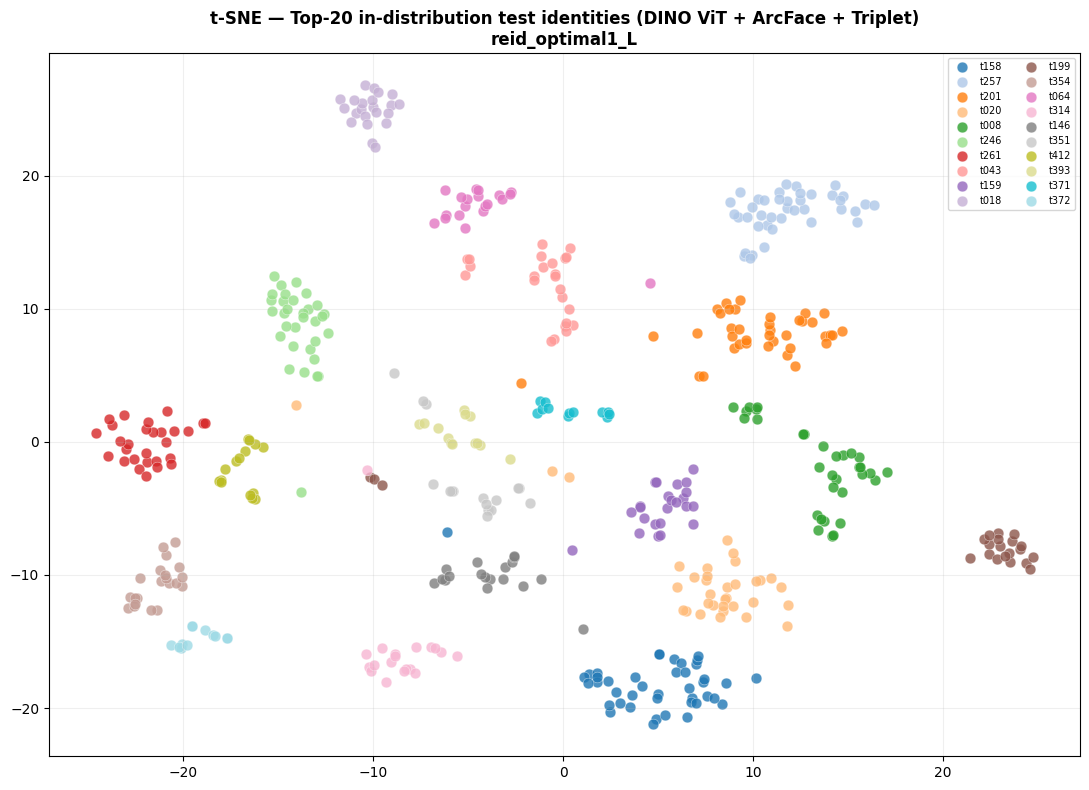
\includegraphics[width=0.85\textwidth]{bab4/tsne2.png}
    \caption{Visualisasi t-SNE untuk 20 identitas penyu teratas pada data pengujian \textit{in-distribution} dengan konfigurasi kombinasi. Setiap warna mewakili satu identitas.}
    \label{fig:tsne_kombinasi}
\end{figure}

%% ============================================================
\section{Pengujian Generalisasi Lintas-Dataset pada SeaTurtleID2022}
\label{sec:pengujian_cross_dataset}
%% ============================================================

%% PERINGATAN: prosedur di bawah kini single-view (tanpa TTA) agar konsisten dengan
%% Subbab protokol evaluasi. Seluruh angka dan gambar bagian ini masih berasal dari run
%% ber-TTA 6-view dan WAJIB di-re-run tanpa TTA sebelum finalisasi:
%% tab:crossdataset_retrieval_only, tab:crossdataset_seaturtleid2022,
%% tab:crossdataset_background_class, tsne3.png, score_dist_threshold.png,
%% score_dist_background.png, cross_query_bottom.png, cross_query_top.png,
%% seluruh rentang skor yang dikutip, dan ROC-AUC 0.77-0.79.

Bagian ini menguji kemampuan generalisasi model ke dataset penyu laut lain di luar
domain pelatihannya. Model dengan \textit{checkpoint} konfigurasi kombinasi
(\textit{backbone} ViT-L/16 DINOv3) diterapkan pada dataset \textbf{SeaTurtleID2022}
tanpa pelatihan ulang. Rangkaian pengujian disusun menaik dari yang paling
mudah ke yang paling menuntut, sehingga setiap tahap mengisolasi satu variabel:

\begin{enumerate}
    \item \textbf{Identifikasi tanpa penolakan.} Seluruh \textit{query} dijamin
          memiliki pasangan di galeri, sehingga yang diuji semata-mata kualitas
          \textit{embedding}.
    \item \textbf{Identifikasi dengan penolakan melalui \textit{threshold} global.}
          Sistem harus menolak \textit{query} dari individu tak terdaftar menggunakan
          satu ambang skor mutlak.
    \item \textbf{Identifikasi dengan penolakan melalui \textit{background class}.}
          Tugas penolakan yang sama, tetapi keputusannya bersifat relatif terhadap
          prototipe individu tak dikenal.
\end{enumerate}

Susunan tersebut memisahkan dua sumber kegagalan yang mungkin terjadi, yaitu apakah
keterbatasan berasal dari kualitas representasi model, atau dari mekanisme pengambilan
keputusan yang bekerja di atas representasi tersebut. Temuan utama seluruh bagian ini
dapat diringkas menjadi tiga poin yang dibuktikan secara berurutan:

\begin{enumerate}
    \item \textbf{Embedding tergeneralisasi dengan penurunan yang terukur.} Pada
          identifikasi tanpa penolakan, model mencapai Rank-1 sebesar 81.1\% dan Rank-5
          sebesar 97.2\% pada dataset baru. Nilai tersebut memang lebih rendah 9.3 poin
          persentase dibanding performa \textit{in-distribution} konfigurasi kombinasi
          (Rank-1 90.4\%), tetapi masih berada pada tingkat yang memadai dan bahkan
          melampaui konfigurasi acuan pada domain aslinya (78.3\%). Kapasitas
          diskriminatif model karenanya bukan merupakan sumber keterbatasan pada skenario
          berpenolakan.
    \item \textbf{Kedua mekanisme penolakan bermuara pada titik operasi yang nyaris
              sama.} Baik \textit{threshold} global sebagai aturan mutlak maupun
          \textit{background class} sebagai aturan relatif menghasilkan
          \textit{trade-off} yang hampir identik, yaitu penolakan individu tak dikenal
          yang nyaris sempurna, dengan konsekuensi penolakan keliru terhadap sekitar
          42\% \textit{query} terdaftar yang valid. Penggantian aturan keputusan hampir
          tidak menggeser titik operasi.
    \item \textbf{Akar persoalan bersifat fundamental pada level skor.} Separabilitas
          skor \textit{registered} terhadap \textit{unregistered} hanya moderat, dengan
          ROC-AUC $\approx 0{.}77$ hingga $0{.}79$. Keterbatasan tersebut membatasi
          seluruh aturan keputusan yang mungkin diterapkan. Aturan relatif yang secara
          rancangan lebih kompleks tidak menghasilkan pemisahan yang lebih baik
          dibandingkan \textit{cosine similarity} sederhana.
\end{enumerate}

\subsection{Prosedur Pengujian}
\label{subsec:openset_prosedur}

Seluruh skenario menggunakan konstruksi galeri dan ekstraksi \textit{embedding} yang
sama, dan perbedaannya hanya terletak pada mekanisme penolakan \textit{unregistered}.

\paragraph{Konstruksi galeri dan query.} Sebanyak 25 identitas dipilih secara acak dari
SeaTurtleID2022 sebagai identitas terdaftar (\textit{registered}). Setiap citra
di-\textit{crop} pada area kepala agar konsisten dengan \textit{preprocessing}
pelatihan. Untuk tiap identitas, 3 citra dipilih secara acak sebagai galeri ($N_G=3$) dan
sisanya menjadi \textit{query}. Galeri disusun per identitas lalu di-\textit{mean-pool}
menjadi satu vektor prototipe yang di-L2-\textit{normalize}. Untuk skenario berpenolakan,
ditambahkan 5 identitas yang sengaja tidak dimasukkan ke galeri (\textit{unregistered}).

\paragraph{Ekstraksi embedding.} Setiap citra diembed dengan \textit{backbone}
ViT-L/16 DINOv3 melalui satu kali lintasan maju atas citra yang telah di-\textit{resize},
kemudian vektor keluarannya di-L2-\textit{normalize}. Prosedur tersebut identik dengan
protokol inferensi pada evaluasi \textit{in-distribution} (Subbab~\ref{subsec:protokol_evaluasi}),
sehingga penurunan performa yang teramati pada bagian ini dapat diatribusikan sepenuhnya
pada pergantian domain, dan bukan pada perbedaan protokol inferensi. \textit{Retrieval}
dihitung dengan \textit{cosine similarity}, dengan opsi \textit{k-reciprocal re-ranking}
($k_1{=}20$, $k_2{=}6$, $\lambda_{\text{rr}}{=}0{.}3$).

\paragraph{Mekanisme penolakan.} Pada skenario berpenolakan, sistem harus memutuskan
apakah sebuah \textit{query} berasal dari identitas terdaftar atau tidak.
\begin{itemize}
    \item \textbf{Threshold global (absolut).} Skor \textit{cosine top-1} terhadap
          galeri dibandingkan terhadap satu ambang tunggal (\textit{Unreg Threshold}).
          Apabila skor berada di bawah ambang, \textit{query} ditandai sebagai
          \textit{Unregistered}. Ambang di-\textit{tune} secara otomatis dengan
          memaksimalkan Youden's J ($\mathit{TPR}-\mathit{FPR}$).
    \item \textbf{Background class (relatif).} Ditambahkan himpunan prototipe
          \textit{background}, yaitu citra penyu di luar 25 identitas galeri, yang
          diambil dari sumber citra terpisah dan dipertahankan sebagai banyak prototipe
          (metode \texttt{samples}, bukan diringkas menjadi satu vektor) agar mewakili
          keragaman individu tak dikenal. Untuk tiap \textit{query} dihitung skor
          keputusan relatif
          \[
              s = s_{\text{reg}} - s_{\text{bg}},
          \]
          yaitu selisih antara kemiripan \textit{top-1} terhadap galeri
          ($s_{\text{reg}}$) dan kemiripan maksimum terhadap prototipe \textit{background}
          ($s_{\text{bg}}$). \textit{Query} diterima sebagai \textbf{Registered} apabila
          $s \geq \textit{margin}$. Karena $s_{\text{bg}}$ dihitung ulang pada setiap
          \textit{query}, skor tersebut menormalisasi \textit{hub identity}, yaitu
          identitas galeri yang mirip terhadap hampir semua citra. \textit{Margin}
          di-\textit{tune} secara otomatis dengan kriteria \texttt{bounded\_frr}
          (\textit{false-reject rate} $\leq 0{.}10$).
\end{itemize}

% VERIFIKASI: pastikan sumber background memang folder terpisah. Bila yang terpakai adalah
% fallback (menyisihkan 50% citra identitas unregistered), jumlah query unregistered pada
% skema background tidak mungkin tetap 49 dan tabel harus dikoreksi.
Karena prototipe \textit{background} diambil dari sumber citra yang terpisah dan tidak
mengambil satu pun citra uji, kedua skema penolakan dievaluasi pada himpunan \textit{query}
yang identik, yaitu 266 citra, sehingga perbandingan keduanya bersifat langsung dan setara.

\subsection{Kualitas Embedding}
\label{subsec:openset_retrieval_only}

Skenario ini hanya berisi 25 identitas terdaftar dan mengasumsikan setiap \textit{query}
pasti memiliki pasangan di galeri, yaitu tanpa individu tak terdaftar dan tanpa mekanisme
penolakan. Hasilnya murni menguji apakah \textit{embedding} model tetap diskriminatif pada
dataset baru.

\begin{table}[H]
    \centering
    \caption{Performa retrieval murni pada query dari identitas terdaftar (tanpa penolakan)}
    \label{tab:crossdataset_retrieval_only}
    \renewcommand{\arraystretch}{1.25}
    \begin{tabular}{lc}
        \hline
        \textbf{Metrik}                     & \textbf{Nilai} \\
        \hline
        Jumlah identitas terdaftar (galeri) & 25             \\
        Citra galeri per identitas ($N_G$)  & 3              \\
        Jumlah \textit{query}               & 217            \\
        Rank-1                              & 81.1\%         \\
        Rank-5                              & 97.2\%         \\
        \hline
    \end{tabular}
\end{table}

Model mencapai Rank-1 sebesar 81.1\% dan Rank-5 sebesar 97.2\% pada dataset yang tidak
digunakan saat pelatihan. Nilai tersebut lebih rendah 9.3 poin persentase dibanding hasil
\textit{in-distribution} konfigurasi kombinasi (Rank-1 90.4\%), sehingga generalisasi
lintas-dataset jelas disertai biaya performa. Namun penurunan tersebut tidak bersifat
katastrofik. Rank-5 sebesar 97.2\% bahkan melampaui Rank-5 \textit{in-distribution}
konfigurasi kombinasi sebesar 96.6\%, dan Rank-1-nya masih berada di atas konfigurasi
acuan pada domain aslinya sebesar 78.3\%. Karena protokol inferensinya identik dengan
evaluasi \textit{in-distribution}, selisih 9.3 poin persentase tersebut dapat
diatribusikan pada pergantian domain semata. Hal ini membuktikan secara langsung bahwa
\textit{embedding} DINOv3 hasil \textit{fine-tuning} tergeneralisasi lintas-dataset.

\begin{figure}[H]
    \centering
    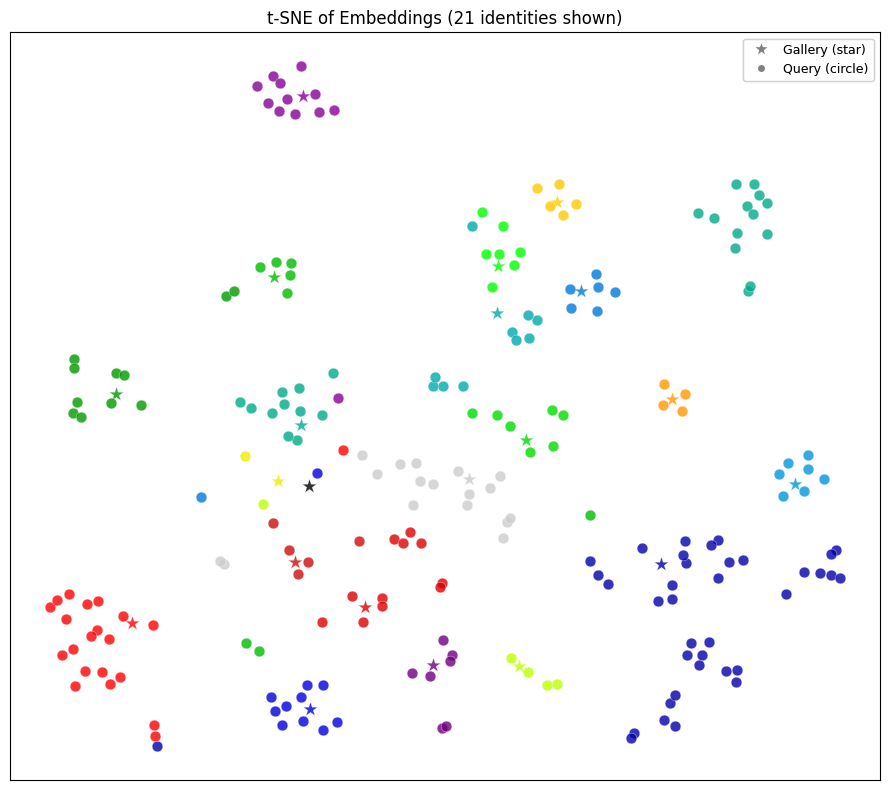
\includegraphics[width=0.85\textwidth]{bab4/tsne3.png}
    \caption{Visualisasi t-SNE vektor \textit{embedding} pada identitas SeaTurtleID2022
        (lintas-dataset, tanpa pelatihan ulang). Bintang menandai prototipe galeri hasil
        \textit{mean-pooling} $N_G=3$ citra, lingkaran menandai citra \textit{query}.
        Setiap warna mewakili satu identitas.}
    \label{fig:tsne_crossdataset}
\end{figure}
% VERIFIKASI: caption lama menyebut 21 identitas, sementara teks menyebut 25 identitas
% terdaftar. Tentukan jumlah identitas yang benar-benar diplot dan cantumkan angkanya.

Gambar~\ref{fig:tsne_crossdataset} memvisualisasikan ruang \textit{embedding} yang
dihasilkan pada dataset lintas-domain tersebut. Struktur yang tampak menjelaskan angka
pada Tabel~\ref{tab:crossdataset_retrieval_only} sekaligus mengantisipasi kegagalan yang
muncul pada skenario berpenolakan.

Klaster tetap terbentuk, tetapi dengan kerapatan yang lebih longgar. Mayoritas identitas
masih membentuk kelompok yang terpisah secara visual dengan prototipe galeri berada di
dalam sebaran \textit{query}-nya sendiri. Struktur inilah yang menopang Rank-1 sebesar
81.1\% dan Rank-5 sebesar 97.2\%. Namun dibandingkan Gambar~\ref{fig:tsne_kombinasi} pada
data \textit{in-distribution}, klaster pada gambar tersebut lebih renggang secara
\textit{intra-class} dan jarak antar-klasternya lebih sempit, konsisten dengan turunnya
Rank-1 dari 90.4\% menjadi 81.1\%. Dengan demikian representasi model tergeneralisasi ke
domain baru, namun disertai penurunan kualitas yang terukur.

\subsection{Identifikasi dengan Penolakan}
\subsubsection{Threshold Global}
\label{subsec:openset_threshold}

Skenario nyata dapat menerima citra individu yang belum pernah didaftarkan. Dengan
penambahan 5 identitas \textit{unregistered}, total \textit{query} menjadi 266, yaitu 217
\textit{registered} dan 49 \textit{unregistered}, dan sistem harus menolak \textit{query}
yang tak terdaftar menggunakan \textit{threshold} global.

\begin{table}[H]
    \centering
    \caption{Hasil identifikasi dengan penolakan pada SeaTurtleID2022 memakai threshold global (25 identitas terdaftar, 5 identitas tidak terdaftar)}
    \label{tab:crossdataset_seaturtleid2022}
    \renewcommand{\arraystretch}{1.25}
    \begin{tabular}{ll}
        \hline
        \textbf{Keterangan}                                          & \textbf{Nilai}                          \\
        \hline
        Jumlah identitas terdaftar (galeri)                          & 25                                      \\
        Citra galeri per identitas ($N_G$)                           & 3                                       \\
        Jumlah identitas tidak terdaftar (baru)                      & 5                                       \\
        \textit{Unregistered threshold} (otomatis, maks. Youden's J) & 0{.}9122                                \\
        Jumlah citra \textit{query}                                  & 266 (terdaftar=217, tidak terdaftar=49) \\
        Akurasi identifikasi                                         & 63.5\%                                  \\
        \textit{Registered} Rank-1 (dengan penolakan)                & 55.3\%                                  \\
        \textit{False-reject rate}                                   & 43.4\%                                  \\
        \textit{Unregistered recall}                                 & 100.0\%                                 \\
        \textit{False-accept rate}                                   & 0.0\%                                   \\
        \hline
    \end{tabular}
\end{table}

Ketika penolakan diaktifkan, \textit{Registered} Rank-1 turun dari 81.1\% pada skenario
tanpa penolakan menjadi 55.3\%. Penurunan tersebut bukan merupakan akibat memburuknya
\textit{embedding}, karena kemampuan \textit{ranking} model tidak berubah sama sekali di
antara kedua skenario. Yang berubah hanyalah keberadaan mekanisme penolakan yang
ditempatkan sebelum proses \textit{ranking}. Sumbernya terbaca jelas dari FRR sebesar
43.4\%, yaitu hampir separuh \textit{query} yang sebenarnya terdaftar ditolak sebagai
\textit{Unregistered} sebelum sempat diperingkat.

\begin{figure}[H]
    \centering
    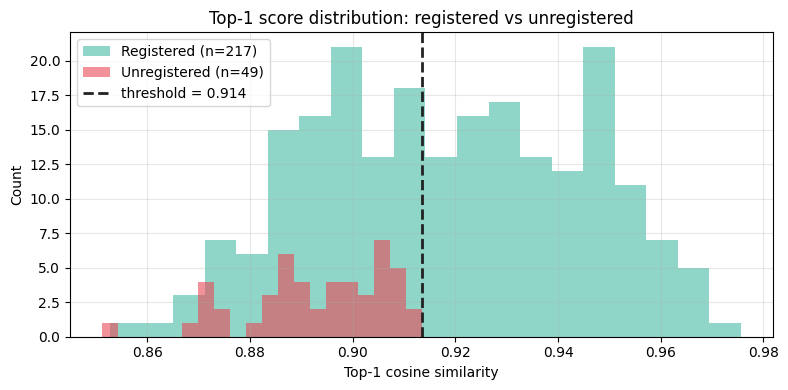
\includegraphics[width=\textwidth]{bab4/score_dist_threshold.png}
    \caption{Distribusi skor \textit{top-1 cosine similarity} terhadap galeri untuk
        \textit{query} terdaftar ($n=217$) dan tidak terdaftar ($n=49$) pada
        SeaTurtleID2022. Garis putus-putus menandai ambang penolakan hasil
        penyetelan otomatis (maks. Youden's J).}
    \label{fig:score_dist_threshold}
\end{figure}

Gambar~\ref{fig:score_dist_threshold} memperlihatkan distribusi skor yang menjadi dasar
seluruh keputusan penolakan pada skema tersebut. Angka-angka pada
Tabel~\ref{tab:crossdataset_seaturtleid2022} merupakan konsekuensi geometris yang dapat
dibaca langsung dari gambar tersebut.

Seluruh skor, baik terdaftar maupun tidak,
terkurung dalam pita $\approx 0{.}85$ hingga $0{.}98$, dan tidak terdapat satu pun
\textit{query} yang skor \textit{top-1}-nya jatuh di bawah 0.85. Artinya, sebuah citra
penyu yang identitasnya sama sekali tidak ada di galeri tetap memperoleh kemiripan
\textit{cosine} sekitar 0.90 terhadap prototipe individu lain. Konsentrasi tersebut
berasal dari struktur data itu sendiri, yaitu seluruh citra berbagi struktur yang nyaris
identik berupa kepala penyu pada latar bawah air, sehingga \textit{embedding} menempati
kerucut sempit pada \textit{hypersphere} dan kemiripan \textit{cosine} antara dua citra
sembarang sudah tinggi sebelum informasi identitas ikut diperhitungkan. Konsekuensinya,
sinyal diskriminatif yang tersedia bagi mekanisme penolakan hanya menempati rentang
selebar $\approx 0{.}13$, jauh lebih sempit dari rentang teoretis \textit{cosine}.

Pola pada
gambar tersebut bukan berupa dua distribusi yang bergeser dan bertumpang tindih pada
tepinya, melainkan distribusi \textit{unregistered} yang seluruhnya tertanam di dalam ekor
bawah distribusi \textit{registered}. Tidak terdapat satu pun \textit{query} tak terdaftar
yang melampaui ambang, sehingga FAR sebesar 0.0\% dan \textit{unregistered recall} sebesar
100.0\% pada Tabel~\ref{tab:crossdataset_seaturtleid2022} dapat diperkirakan sebelumnya,
karena ambang memang ditempatkan tepat pada batas atas sebaran skor mereka. Perlu
ditekankan bahwa \textit{recall} sebesar 100.0\% tersebut diperoleh dari hanya 49
\textit{query} tak terdaftar dan pada ambang yang di-\textit{tune} pada himpunan yang sama,
sehingga tidak dapat dibaca sebagai jaminan penolakan sempurna pada data baru. Karena
distribusi \textit{registered} juga menempati pita yang sama, setiap ambang yang cukup
tinggi untuk menyingkirkan seluruh \textit{unregistered} pasti ikut menyingkirkan sebagian
besar \textit{registered}. FRR sebesar 43.4\% karenanya merupakan konsekuensi langsung dari
struktur distribusi tersebut, dan bukan akibat penyetelan ambang yang keliru.

Kriteria
$J=\mathit{TPR}-\mathit{FPR}$ menyeimbangkan proporsi ternormalisasi, dan bukan cacah
mentah. Pada pita tumpang tindih $\approx 0{.}88$ hingga $0{.}91$, meskipun cacah
\textit{registered} per \textit{bin} tampak lebih tinggi secara visual, mayoritas dari
hanya 49 \textit{query} tak terdaftar terkonsentrasi pada pita tersebut, sementara 217
\textit{query} terdaftar tersebar hingga 0.98. Kerapatan ternormalisasi
\textit{unregistered} pada pita tersebut karenanya lebih tinggi daripada
\textit{registered}. Setiap penurunan ambang di wilayah tersebut menambah FPR lebih cepat
daripada menambah TPR, sehingga $J$ maksimum tercapai persis pada titik FPR $=0$. Optimum
tersebut bersifat \textit{corner solution}, yaitu terpilih bukan karena merupakan kompromi
yang baik, melainkan karena tidak tersedia kompromi yang lebih baik.

\subsubsection{Background Class}
\label{subsec:openset_background}

Pendekatan \textit{threshold} bersifat \textit{post-hoc}, yaitu satu ambang mutlak di atas
skor \textit{cosine} yang terpisah dari proses \textit{retrieval}. Sebagai alternatifnya,
penolakan dijadikan bagian dari kompetisi \textit{retrieval} itu sendiri melalui
\textit{background class}, yaitu sebuah \textit{query} ditolak apabila prototipe
\textit{background} mengungguli kandidat galeri terbaiknya
($s = s_{\text{reg}} - s_{\text{bg}} < \textit{margin}$).

\begin{table}[H]
    \centering
    \caption{Hasil identifikasi dengan penolakan memakai penambahan background class pada galeri}
    \label{tab:crossdataset_background_class}
    \renewcommand{\arraystretch}{1.25}
    \begin{tabular}{ll}
        \hline
        \textbf{Keterangan}                                     & \textbf{Nilai}                          \\
        \hline
        Jumlah identitas terdaftar (galeri)                     & 25                                      \\
        Citra galeri per identitas ($N_G$)                      & 3                                       \\
        Metode prototipe                                        & \texttt{samples}                        \\
        \textit{Margin} keputusan (auto, \texttt{bounded\_frr}) & $+0{.}0148$                             \\
        Jumlah citra \textit{query}                             & 266 (terdaftar=217, tidak terdaftar=49) \\
        Akurasi identifikasi                                    & 64.3\%                                  \\
        \textit{Registered} Rank-1 (dengan penolakan)           & 56.7\%                                  \\
        \textit{False-reject rate}                              & 41.9\%                                  \\
        \textit{Unregistered recall}                            & 98.0\%                                  \\
        \textit{False-accept rate}                              & 2.0\%                                   \\
        \hline
    \end{tabular}
\end{table}

Temuan paling penting dari skema tersebut bukanlah keunggulannya, melainkan kemiripannya
dengan \textit{threshold} global. Karena kedua skema dievaluasi pada himpunan
\textit{query} yang identik sebanyak 266 citra, perbandingannya bersifat langsung.
Meskipun mekanismenya berbeda secara fundamental, yaitu mutlak berbanding relatif,
\textit{background class} bermuara pada titik operasi yang nyaris sama, yaitu
\textit{Registered} Rank-1 sebesar 56.7\% berbanding 55.3\%, FRR sebesar 41.9\% berbanding
43.4\%, \textit{unregistered recall} sebesar 98.0\% berbanding 100.0\%, dan FAR sebesar
2.0\% berbanding 0.0\%. Akurasi identifikasi keduanya pun berdekatan, yaitu 64.3\%
berbanding 63.5\%. Seluruh selisih tersebut berada pada orde satu hingga dua
\textit{query}. Skema relatif tersebut karenanya tidak membuka \textit{trade-off} yang
lebih baik, melainkan hanya mencapai titik operasi yang sama ketatnya melalui jalan yang
berbeda.

Konsistensi tersebut sekali lagi menegaskan bahwa \textit{embedding} tidak pernah menjadi
sumber masalah. Efek seleksi yang sama juga muncul, yaitu di antara \textit{query}
terdaftar yang lolos, akurasi \textit{retrieval} mencapai $0{.}567/(1-0{.}419) \approx
    97{.}6\%$, praktis identik dengan $\approx 97{.}7\%$ pada \textit{threshold} global.
Kedua mekanisme penolakan sama-sama ketat, sehingga sama-sama menyingkirkan kasus sulit
terlebih dahulu dan menyisakan subset \textit{query} yang relatif mudah.

\begin{figure}[H]
    \centering
    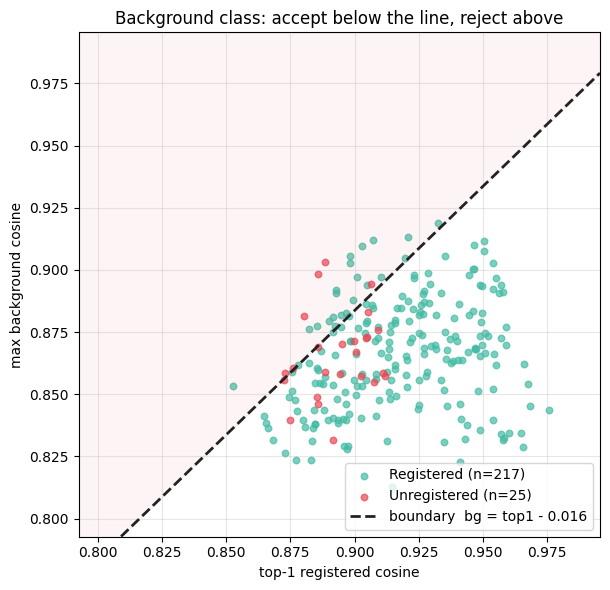
\includegraphics[width=0.8\textwidth]{bab4/score_dist_background.png}
    \caption{Ruang keputusan \textit{background class} pada SeaTurtleID2022. Sumbu
        horizontal menyatakan kemiripan \textit{top-1} terhadap prototipe galeri
        ($s_{\text{reg}}$), sumbu vertikal menyatakan kemiripan maksimum terhadap
        prototipe \textit{background} ($s_{\text{bg}}$). Garis putus-putus adalah batas
        keputusan $s_{\text{bg}} = s_{\text{reg}} - \textit{margin}$; \textit{query} di
        bawah garis diterima sebagai \textit{Registered}, di atas garis ditolak.}
    \label{fig:bg_class_scatter}
\end{figure}

Gambar~\ref{fig:bg_class_scatter} memplot kedua komponen skor keputusan secara terpisah,
sehingga dapat diperiksa berapa besar kontribusi masing-masing terhadap keputusan akhir.
Dari gambar tersebut dapat dibaca alasan mengapa skema relatif ini bermuara pada titik
operasi yang nyaris identik dengan \textit{threshold} global.

Sumbu vertikal tidak membawa informasi diskriminatif. Perbandingan sebaran kedua kelas
pada masing-masing sumbu bersifat menentukan. Pada sumbu horizontal, \textit{query} tak
terdaftar terkonsentrasi pada pita $s_{\text{reg}} \approx 0{.}85$ hingga $0{.}915$
sementara \textit{query} terdaftar terbentang hingga $\approx 0{.}975$, sehingga pemisahan
antar-kelas terjadi di sepanjang sumbu tersebut, persis seperti pada
Gambar~\ref{fig:score_dist_threshold}. Sebaliknya, pada sumbu vertikal kedua kelas
menempati rentang yang praktis berimpit, yaitu $s_{\text{bg}} \approx 0{.}83$ hingga
$0{.}92$, dengan pemusatan yang nyaris sama. Nilai $s_{\text{bg}}$ juga tidak menunjukkan
ketergantungan yang kuat terhadap $s_{\text{reg}}$, karena untuk hampir seluruh rentang
$s_{\text{reg}}$ sebaran $s_{\text{bg}}$ tetap serupa. Dengan demikian $s_{\text{bg}}$
tidak membawa informasi mengenai apakah sebuah \textit{query} terdaftar atau tidak. Skor
keputusan $s = s_{\text{reg}} - s_{\text{bg}}$ karenanya secara efektif merupakan
$s_{\text{reg}}$ yang ditambahi komponen derau, dan hal inilah yang menyebabkan aturan
relatif tersebut bermuara pada titik operasi yang sama dengan aturan mutlak.

\subsection{Analisis Kualitatif Lintas Dataset}
Gambar~\ref{fig:cross_query_bottom} dan Gambar~\ref{fig:cross_query_top} menampilkan lima
keputusan paling keliru dan lima keputusan paling tepat pada skema
\textit{background class}, lengkap dengan lima kandidat galeri teratas beserta skor
\textit{cosine}-nya.

\begin{figure}[H]
    \centering
    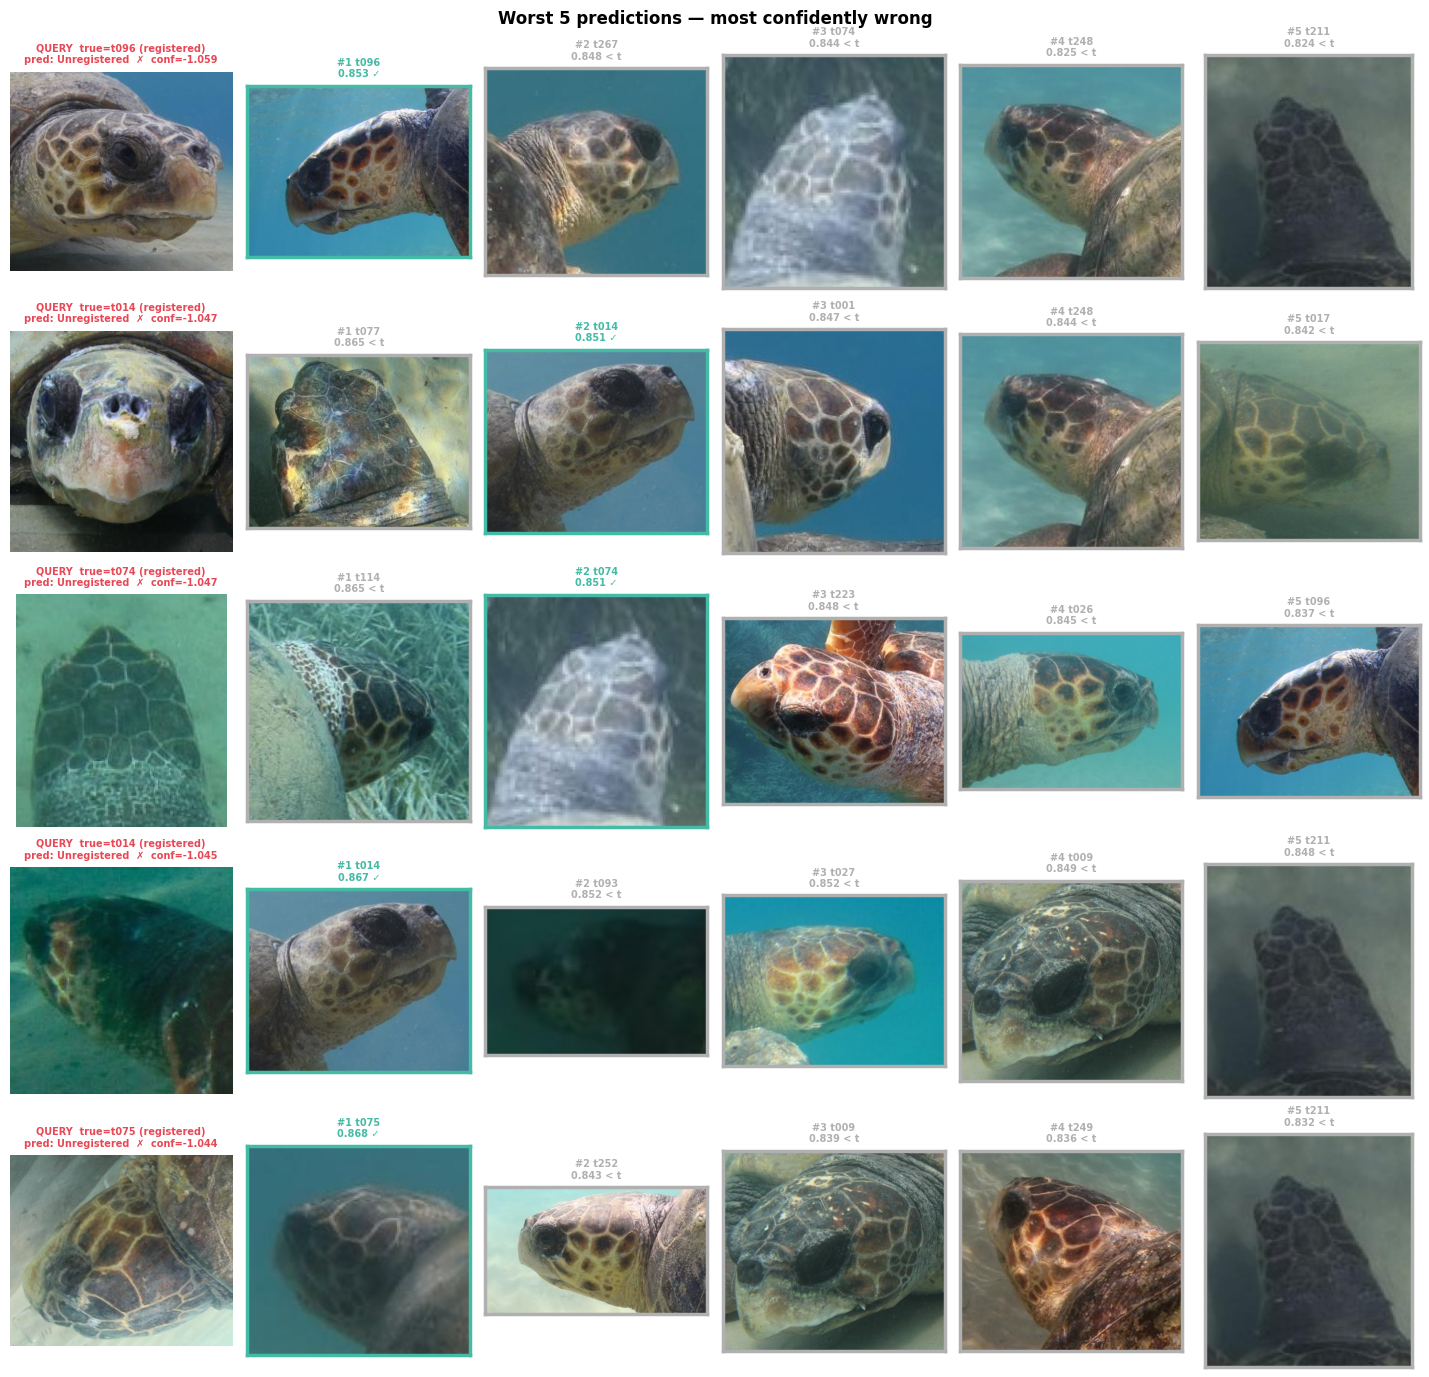
\includegraphics[width=\textwidth]{bab4/cross_query_bottom.png}
    \caption{Lima keputusan paling keliru pada skema \textit{background class}
        (SeaTurtleID2022). Kolom pertama adalah citra \textit{query} beserta identitas
        sebenarnya dan prediksi sistem; kolom berikutnya adalah lima kandidat galeri
        teratas terurut menurun berdasarkan \textit{cosine similarity}. Penanda hijau
        menunjukkan kandidat dengan identitas yang benar.}
    \label{fig:cross_query_bottom}
\end{figure}

\begin{figure}[H]
    \centering
    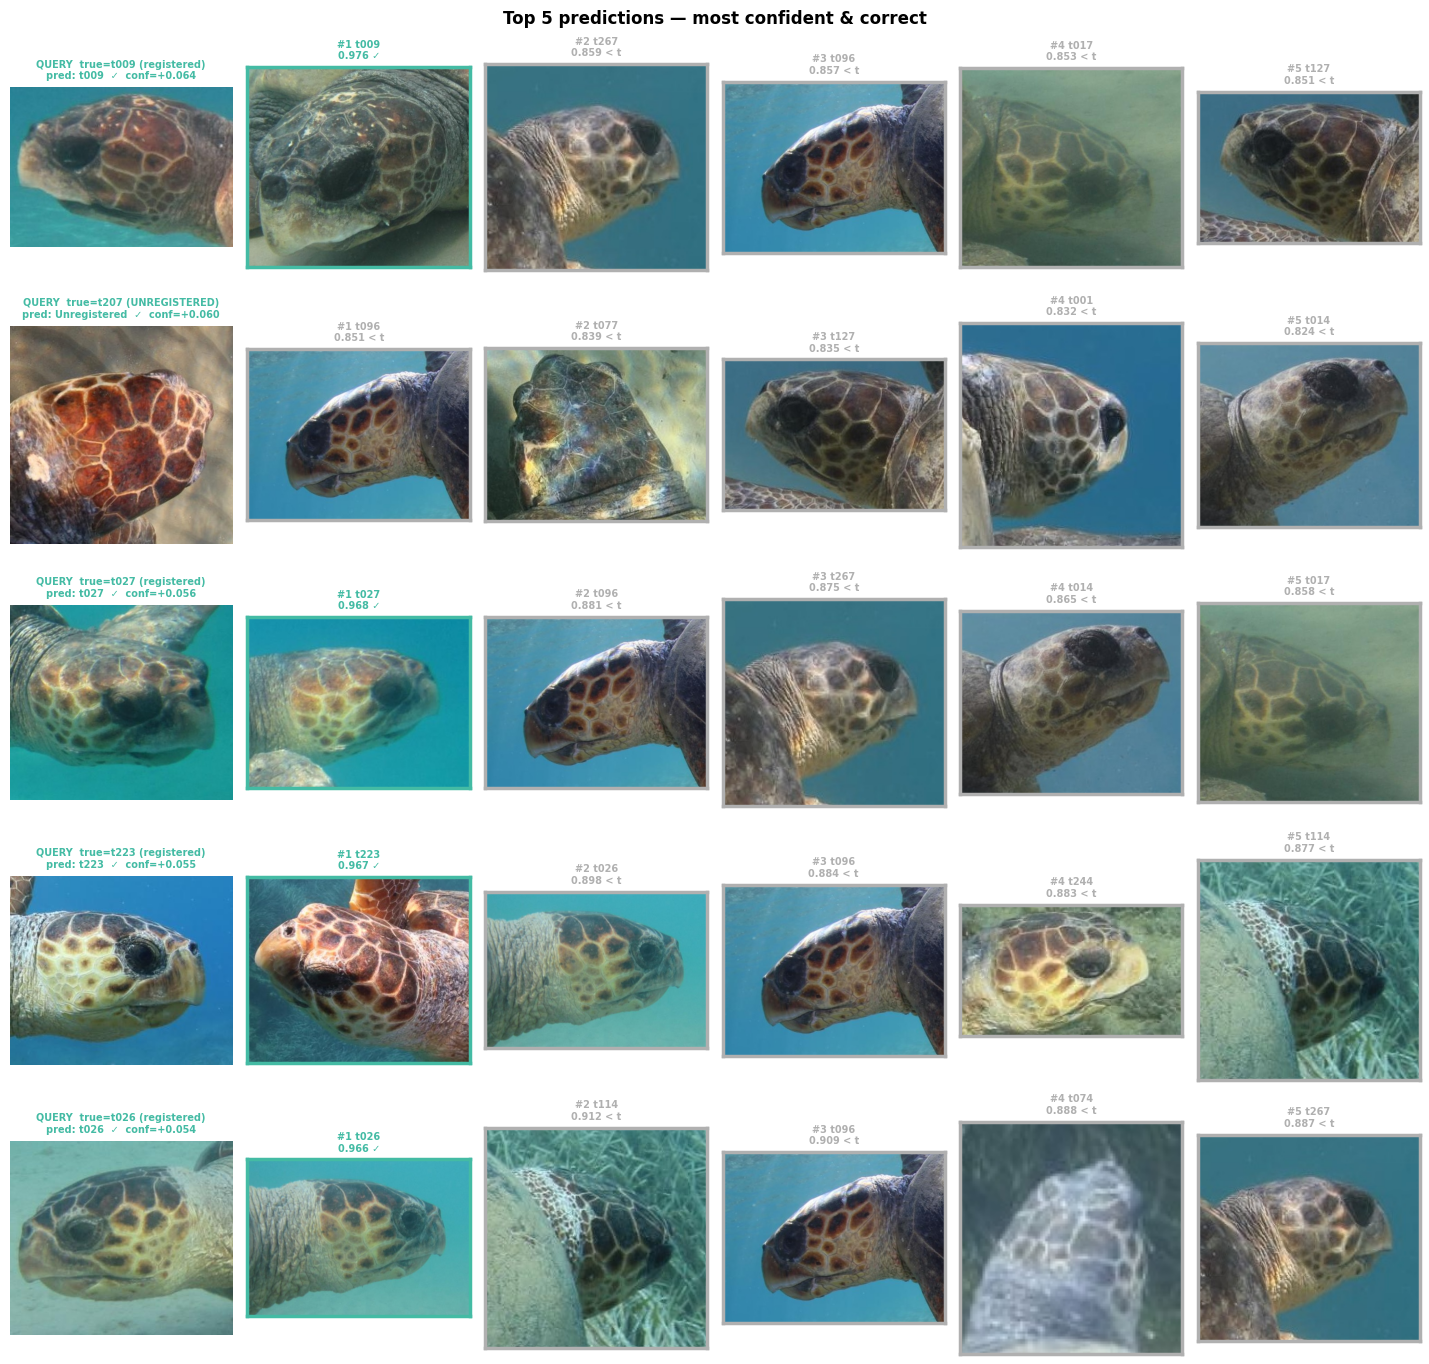
\includegraphics[width=\textwidth]{bab4/cross_query_top.png}
    \caption{Lima keputusan paling tepat pada skema \textit{background class}
        (SeaTurtleID2022), dengan konvensi penyajian yang sama dengan
        Gambar~\ref{fig:cross_query_bottom}.}
    \label{fig:cross_query_top}
\end{figure}

Dua hal dapat dianalisis dari Gambar~\ref{fig:cross_query_bottom}, dan keduanya memperkuat
kesimpulan bahwa keterbatasan sistem terletak pada mekanisme keputusan, dan bukan pada
representasi.

Pertama, kelima kegagalan terparah merupakan \textit{query} dari identitas terdaftar
yang ditolak sebagai \textit{Unregistered}, dan tidak satu pun di antaranya merupakan
\textit{false accept}. Komposisi tersebut merupakan wujud visual dari asimetri pada
Tabel~\ref{tab:crossdataset_background_class}, yaitu FRR sebesar 41.9\% berhadapan dengan
FAR sebesar 2.0\%. Kegagalan mekanisme penolakan karenanya tidak bersifat simetris,
melainkan hampir seluruhnya terjadi pada satu arah.

Kedua, dan yang paling menentukan, pada kelima kasus tersebut identitas yang benar tetap
berada di dalam lima kandidat teratas, bahkan tepat pada peringkat-1 untuk tiga di
antaranya, yaitu t096 dengan skor 0.853, t014 dengan skor 0.867, dan t075 dengan skor
0.868. Pada kasus yang secara kuantitatif tergolong paling parah sekalipun, proses
\textit{retrieval} sesungguhnya telah menempatkan jawaban yang benar pada posisi teratas,
dan keputusan penolakanlah yang kemudian membuangnya sebelum peringkat tersebut sempat
dilaporkan. Temuan tersebut menutup kemungkinan bahwa penurunan \textit{Registered} Rank-1
dari 81.1\% menjadi 56.7\% berasal dari melemahnya kualitas \textit{embedding} pada domain
baru.

Perbandingan dengan Gambar~\ref{fig:cross_query_top} memperlihatkan alasan mengapa
mekanisme penolakan tersebut tidak dapat disetel lebih longgar. Keputusan yang tepat
ditandai skor \textit{top-1} pada rentang 0.966 hingga 0.976, terpisah jelas dari kandidat
kedua yang berada di sekitar 0.86 hingga 0.91. Sebaliknya, penolakan yang benar terhadap
identitas tak terdaftar (t207) terjadi ketika skor \textit{top-1}-nya hanya mencapai 0.851.
Perbandingan inilah yang menjadi inti persoalan. Pada kasus gagal di
Gambar~\ref{fig:cross_query_bottom}, skor pencocokan yang benar berada pada rentang 0.851
hingga 0.868, yaitu berimpit dengan skor \textit{top-1} milik \textit{query} t207 yang
identitasnya sama sekali tidak ada di galeri. Sebuah pencocokan yang benar dan sebuah
\textit{query} yang sepenuhnya asing karenanya menghasilkan skor yang praktis tidak dapat
dibedakan. Sistem hanya dapat memutuskan dengan andal ketika \textit{query} memiliki
pasangan galeri berpose serupa yang menghasilkan skor di atas $\approx 0{.}95$, sedangkan
di luar kondisi tersebut seluruh kasus terkonsentrasi pada pita 0.84 hingga 0.88 yang sama.
Inilah dasar konkret dari ROC-AUC $\approx 0{.}77$ hingga $0{.}79$ yang membatasi seluruh
aturan keputusan, sekaligus alasan mengapa penggantian aturan keputusan dari mutlak menjadi
relatif tidak menggeser titik operasi.